\documentclass[10pt]{scrartcl}

\usepackage[margin=2.5cm]{geometry}
\usepackage{microtype}
\usepackage{abstract}
\usepackage[ngerman]{babel}
\usepackage{biblatex}
\addbibresource{quellen.bib}
\usepackage{hyperref}
\usepackage{siunitx}
\sisetup{locale=DE}
\usepackage{amsmath}
\usepackage{amssymb}
\usepackage{graphicx}
\usepackage{subfig}
\usepackage{parskip}

\newcommand{\filepath}[1]{\texttt{#1}}

%%%%%%%%%%%%%%% ABBILDUNGEN
    \usepackage{graphicx}
    \usepackage{float} % Figure "H" Option zur Positionierung
    \usepackage{caption} % Für custom captions
    \captionsetup{textfont={footnotesize}, labelfont={footnotesize, bf}, position=below, format=plain, skip=7pt}
    % \DeclareCaptionOption{parskip}[]{} % Option "parskip" lahmlegen, damit subfig nicht darüber stolpert \usepackage{subfig}
    %%%%%%%% TIKZ
        \usepackage{tikz}
        \usetikzlibrary{matrix, positioning, calc, %
        decorations.pathreplacing, calligraphy, % for curly braces
        plotmarks % für mehr plot marks
        }
        \usepackage{circuitikz} % Schaltplan,Schaltzeichen usw.
        \tikzset{big elko/.style={elko=#1, capacitors/width=0.3}}
        \usepackage{pgfplots} % Plots
        \pgfplotsset{compat=1.18} % Neuste Version nutzen
        \usepackage{adjustbox} % Für Scaling von tikz pictures
    
%%%%%%%%%%%%%%% PROGRAMMAUSSCHNITTE
    \usepackage[newfloat=true]{minted}
    \usepackage{xparse} % Für NewDocumentCommand und -Environment
    \usepackage{varwidth}
    \definecolor{bg}{rgb}{0.95,0.95,0.95}
    \SetupFloatingEnvironment{listing}{name=Programmausschnitt, listname=Programmausschnitte}
    % https://stackoverflow.com/a/1390520
    %                             #1     #2       #3 #4 #5
    \NewDocumentEnvironment{code}{O{0.7} O{julia}  m  m}{%
        \VerbatimEnvironment%
        \begin{listing}[hp]%
            \centering% also for centering
            \begin{varwidth}{#1\textwidth}%
                \begin{minted}[bgcolor=bg, linenos, breaklines,fontsize=\footnotesize]{#2}%
                    } {%
                \end{minted}%
            \end{varwidth}%
            \vspace{-1ex}%
            \caption{#3}%
            \label{#4}%
        \end{listing}%
    }
    \newcommand{\coderef}[1]{Programmausschnitt \ref{#1}}

\usepackage{csquotes}
\usepackage{fancyhdr} % Kopf- und Fußzeilen
% https://tex.stackexchange.com/a/313337
\usepackage{enumitem,amssymb}
\newlist{todolist}{itemize}{2}
\setlist[todolist]{label=$\square$}
\usepackage{pifont}
\newcommand{\cmark}{\ding{51}}%
\newcommand{\xmark}{\ding{55}}%
\newcommand{\todo}{$\square$}
\newcommand{\done}{\rlap{$\square$}{\raisebox{2pt}{\large\hspace{1pt}\cmark}}%
\hspace{-2.5pt}}
\newcommand{\wontfix}{\rlap{$\square$}{\large\hspace{1pt}\xmark}}

\setlist[itemize]{noitemsep}
\setlist[enumerate]{noitemsep}

\usepackage{tabularray}

\newcommand*{\eng}[1]{\textit{#1}}
\newcommand*{\feng}[1]{\eng{#1}}
\newcommand{\lee}{Lee {\itshape et al.} (2022)}

\pgfplotsset{every axis/.append style={
        scaled y ticks = false, 
        scaled x ticks = false, 
        y tick label style={/pgf/number format/.cd, fixed, fixed zerofill,
                            int detect,1000 sep={\;},precision=3},
        x tick label style={/pgf/number format/.cd, fixed, fixed zerofill,
                            int detect, 1000 sep={},precision=3}
    }
}

\usepackage{fontspec}
\newfontfamily\sansemph{Latin Modern Sans} % Für Titel

\begin{document}
\pagenumbering{gobble}
\thispagestyle{empty}

\vspace*{10mm}
\begin{center}
    {\Huge \textbf{\sansemph Analyse der Optimierungsverfahren mechanischer neuronaler Netzwerke}}%
    % \\[2mm]
    % {\Large Sammlung, Verarbeitung und Analyse unserer Gehirnsignale} 
    \\[4mm]
    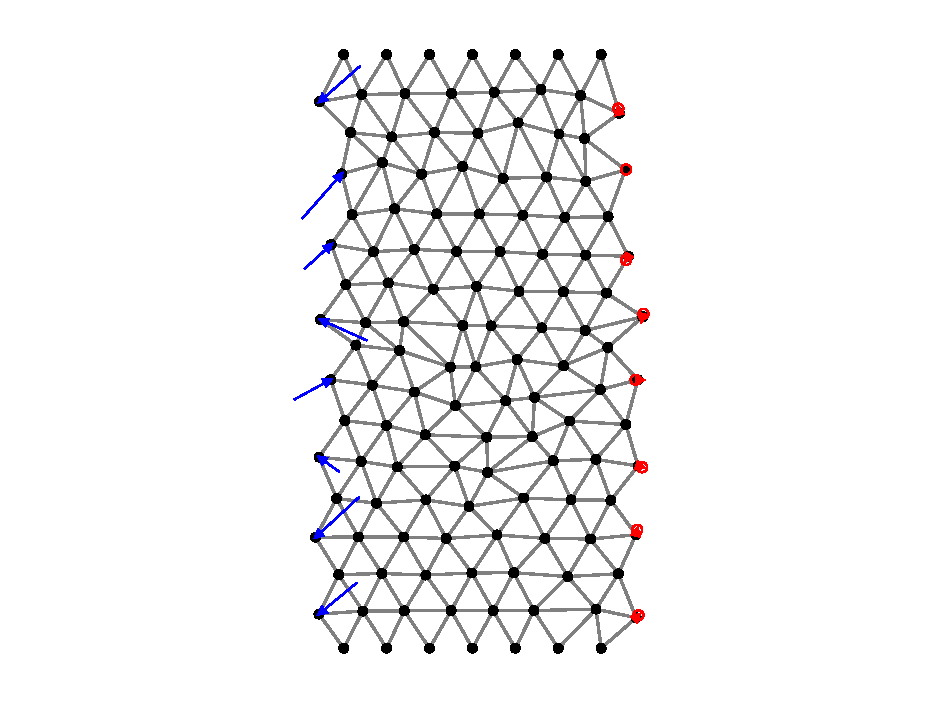
\includegraphics[width=0.8\textwidth]{bilder/test2.pdf} \\[4mm]
    {\huge \textbf{Alexander Reimer \qquad Matteo Friedrich}} \\[1em]
    {\LARGE {Gymnasium Eversten Oldenburg}} \\[1.2ex]
    {\LARGE {Betreuer: Herr Dr. Glade}}
\end{center}

\newpage

\tableofcontents

\section*{Zusammenfassung}

Wir wollen uns mit dem neuen, noch vergleichsweise wenig erforschten Bereich der \feng{mechanical neural networks}, kurz MNNs, beschäftigen.
MNNs sind programmierbare Materialien, welchen verschiedene Verhaltensweisen, wie zum Beispiel ein bestimmtes Verformungsverhalten, antrainiert werden können. Sie bestehen aus Massepunkten (genannt Neuronen), welche durch Federn miteinander verbunden werden. Ihr Verhalten ergibt sich durch die Steifheiten der Federn.
Die grundlegende Annahme von MNNs ist, dass diese Federkonstanten in zukünftigen Materialien einzeln angepasst werden können. 
In Analogie zu künstlichen neuronalen Netzwerken wäre es dann prinzipiell möglich, durch eine geeignet gewählte Konfiguration an Federkonstanten verschiedene Verhaltensweisen auf externe Kräfte anzutrainieren.
Während sich die bisherige Forschung auf die technische, physische Implementation dieser Netzwerke fokussiert hat, wollen wir das Trainingsverfahren optimieren.
Dazu haben wir bereits eine Simulation eines MNNs umgesetzt, die bisher verwendeten Algorithmen (evolutionäres Lernen und Pattern Search) selbst implementiert, sowie mit neuen Parametern ausprobiert und verglichen. 
Dafür haben wir uns jedoch auf die Anwendung dieser Algorithmen in Simulationsrechnungen beschränkt. Die Ergebnisse sollten dennoch einen guten Startpunkt für reale MNNs bieten. Der von uns entwickelte Code ist die erste öffentlich verfügbare Implementation eines MNNs.
Unsere Ergebnisse zeigen, dass MNNs mehrere komplexe Verhaltensweisen lernen können. Diese intelligenten Materialien %TODO
eröffnen vielfältige zukünftige technologische Anwendungsmöglichkeiten. % für die Materialforschung.


\pagestyle{fancy}
\fancyhead{}
\fancyhead[L]{\rightmark}
\fancyhead[R]{JUGEND FORSCHT -- PROJEKTBERICHT}
\pagenumbering{roman}

\newpage

\pagestyle{fancy}
\fancyhead{}
\fancyhead[L]{\rightmark}
\fancyhead[R]{JUGEND FORSCHT -- PROJEKTBERICHT}
\pagenumbering{arabic}

\section{Einleitung}

Inspiration für dieses Projekt ist ein Artikel von 2022 mit dem Titel \enquote{Mechanical neural networks: Architected materials that learn behaviors} von \lee{} \cite{Lee2022}.
%
Es ist der erste uns bekannte veröffentlichte Artikel, der sogenannte \feng{mechanical neural networks}, kurz MNNs, beschreibt -- ein neuer Forschungsbereich, in dem neuronale Netzwerke in der physischen Welt umgesetzt werden (s. Abb. \ref{fig:mnn2-1}).
Im Gegensatz zu bisherigen mathematischen und elektrischen Implementationen handelt es sich hier um eine mechanische, bei der Federn mit variabler Steifheit miteinander verbunden werden.
Abhängig von den Härten der Federn (Federkonstanten) weist das Material unterschiedliche Verhaltensweisen bei Krafteinwirkung auf. 
%
Ein MNN kann also als anpassbares und durch Sensoren sogar lernfähiges Material verwendet werden, welches seinen Bedingungen oder gewünschten Verwendungszwecken angepasst werden kann.
Dazu kann das Material sowohl in einer Simulation als auch physisch, durch Sensoren in den Federn, trainiert werden.

\begin{figure}[htbp!]
    \centering
    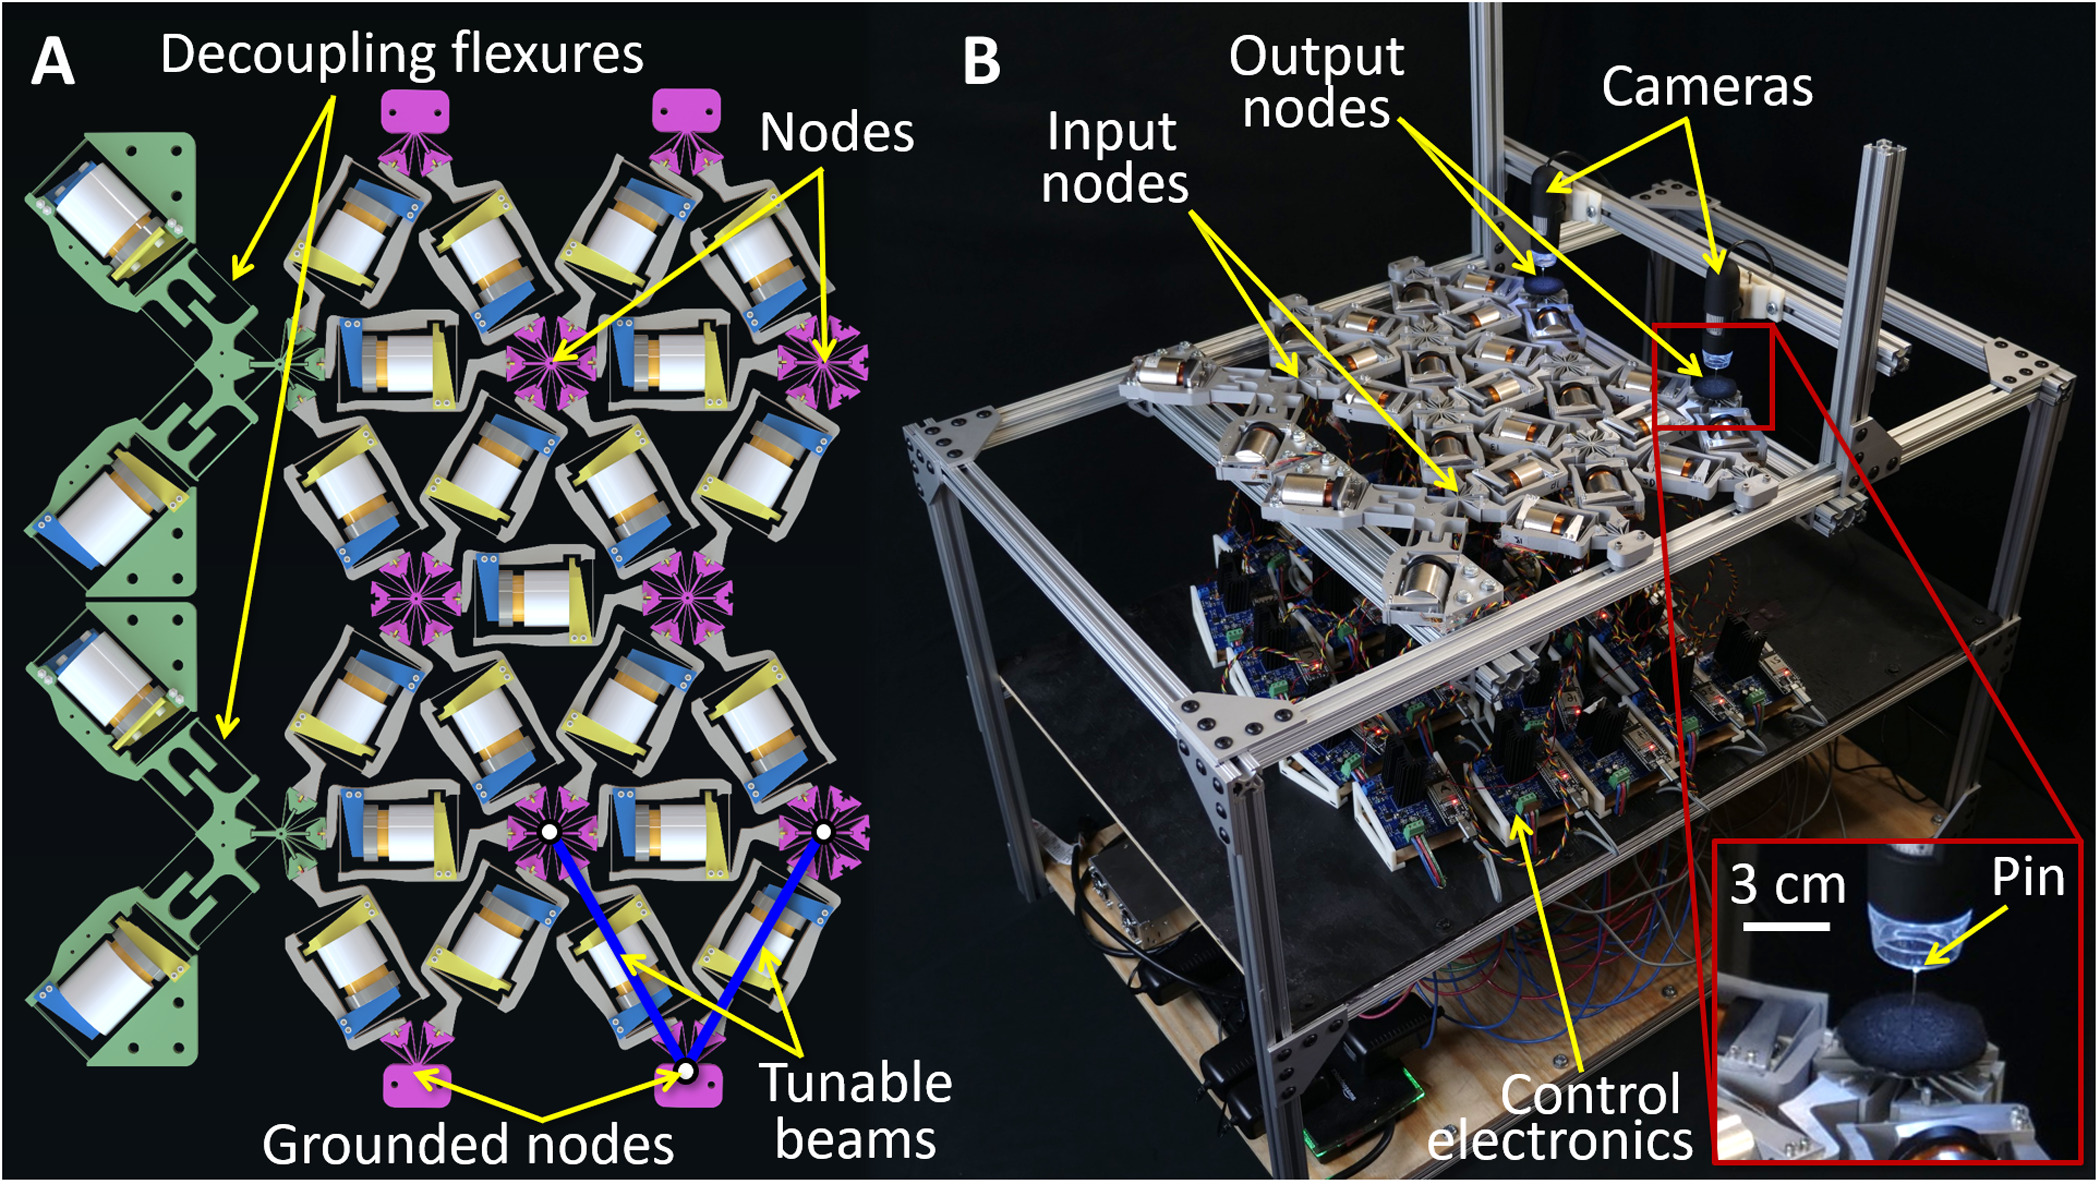
\includegraphics[width=0.65\linewidth]{bilder/mnn2-1.jpg}
    \caption{Mechanische Umsetzung eines MNN (Abb. von \cite{Lee2022})}
    \label{fig:mnn2-1}
\end{figure}

Durch ihre Eigenschaften könnten MNNs viele Verwendungszwecke haben, von der Optimierung von Flugzeugflügeln abhängig von aktuellen Gegebenheiten wie Windstärke und -winkel \cite[2]{Lee2022} über Optimierung der Schockabsorption von Schutzwesten bis zur dynamischen Änderung der Resonanzfrequenz eines Gebäudes zum Schutz gegen Erdbeben \cite[9]{Hopkins2023}.
Wenn es möglich ist, die Resonanz auf Schwingungen eines MNNs zu trainieren, könnte man dies auch für einbruchsichere Brücken oder vielleicht sogar bessere Musikinstrumente nutzen.

In diesem Projekt wollen wir verschiedene Optimierungsalgorithmen für MNNs vergleichen.
% und analysieren, wie viele verschiedene Verhaltensweisen gleichzeitig gelernt werden können. 
Da wir nichts passendes finden konnten, wollen wir zuerst eine eigene Programmbibliothek zur Simulation, Optimierung, Bewertung und Visualisierung von MNNs erstellen.
Diese soll nutzerfreundlich und öffentlich sein, damit wir und andere sie als Basis für weiterführende Projekte nutzen können.

Zur Bewertung der Optimierungsalgorithmen und -parameter sollen MNNs simuliert werden.
Ziel dieses Projektes ist es aufgrund des hohen Aufwands nicht, ein MNN selbst physisch umzusetzen;
es wird jedoch davon ausgegangen, dass ein Vergleich der Verfahren in einer Simulation auch korrekte Aussagen über das physische Trainieren liefern wird und ein \enquote{Vortrainieren} eines physischen MNN mit einer Simulation die Gesamtzeit des Trainierens verkürzen kann, somit also auch die in einer Simulation verwendeten Optimierungsverfahren relevant sind.

% \begin{figure}
%     \centering
%     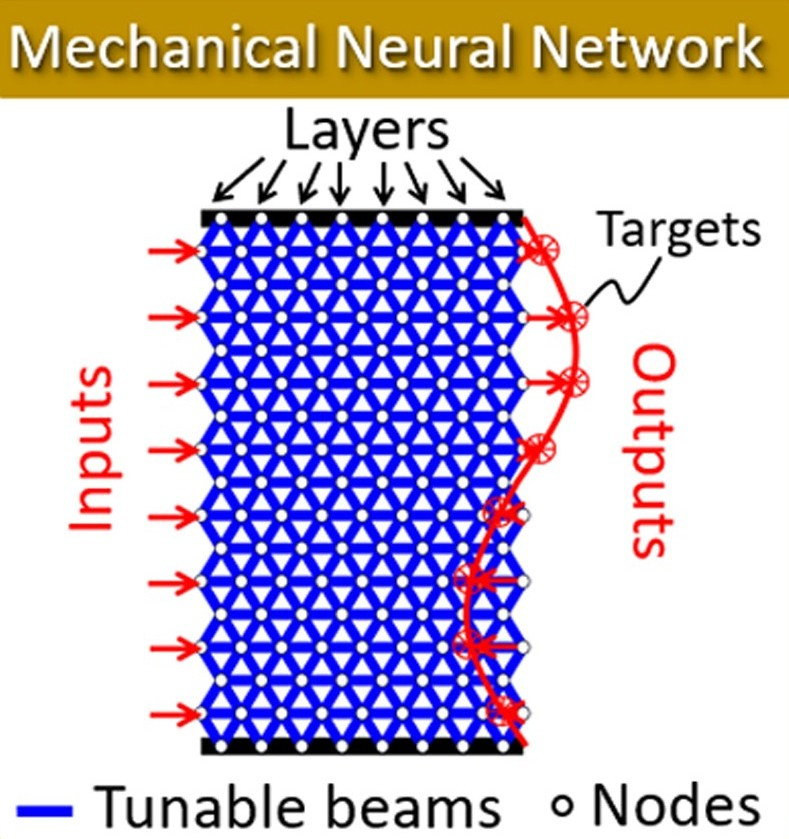
\includegraphics[width=0.4\linewidth]{bilder/mnn1-1.jpg}
%     \caption{Repräsentation eines MNN (von \cite{Lee2022})}
%     \label{fig:mnn1-1}
% \end{figure}
\newpage
\section{Hintergrund und theoretische Grundlagen}

Mechanische Neuronale Netzwerke (MNNs) scheinen künstlichen neuronalen Netzwerken (\eng{artificial neural networks}, kurz ANNs) in ihrem Aufbau zwar ähnlich (vgl. Abb. \ref{fig:dense_nn} und \ref{fig:mnn2-1}), unterscheiden sich in ihrer Funktionsweise und Umsetzung jedoch stark.

\begin{figure}[H]
    \def\layersep{6cm}
    \def\biasDist{0.6}
    \centering
    \adjustbox{scale=0.9}{%
    \begin{tikzpicture}[
        % scale=1.2,
        shorten >=1pt,->,draw=black!70, node distance=\layersep,
        neuron/.style={circle,fill=black!25,minimum size=20,inner sep=0},
        edge/.style 2 args={pos={(mod(#1+#2,2)+1)*0.33}, font=\tiny},
        distro/.style 2 args={
            edge={#1}{#2}, node contents={}, minimum size=0.6cm, path picture={\draw[double=orange,white,thick,double distance=1pt,shorten >=0pt] plot[variable=\t,domain=-1:1,samples=51] ({\t},{0.2*exp(-100*(\t-0.05*(#1-1))^2 - 3*\t*#2))});}
          },
        weight/.style 2 args={
            edge={#1}{#2}, node contents={\pgfmathparse{0.35*#1-#2*0.15}\pgfmathprintnumber[fixed]{\pgfmathresult}}, fill=white, inner sep=2pt
          }
      ]
    % Input layer
    \foreach \y in {1,...,2}
        \node[neuron, fill=green!40] (i\y) at (0,\y+1) {$i_\y$};
    \node[neuron, fill=orange!40, above=\biasDist of i2] (b1) {$b_1$};
    % Hidden layer
    \foreach \y in {1,...,4}
        \path node[neuron, fill=blue!40] (h\y) at (\layersep,\y) {$h_\y$};
    \node[neuron, fill=orange!40, above=\biasDist of h4] (b2) {$b_2$};
    % Output node
    \node[neuron, fill=red!40] (o) at (2*\layersep,2.5) {$O$};
    
    % Connect every node in the input layer with every node in the hidden layer.
    \foreach \source in {1,...,2}
        \foreach \dest in {1,...,4}
            \path (i\source) edge (h\dest);
    % Connect bias in the input layer with every node in the hidden layer.
    \foreach \dest in {1,...,4}
        \path[red!20] (b1) edge (h\dest);
    % Connect every node in the hidden layer with the output layer
    \foreach \source in {1,...,4}
        \path (h\source) edge (o);
    % Connect bias in the hidden layer with the output layer
    \path[red!20] (b2) edge (o);
        
    % Draw weights for all regular edges.
    \foreach \i in {1,...,2}
        \foreach \j in {1,...,4}
            \path (i\i) -- (h\j) node[weight={\i}{\j}];
    \foreach \i in {1,...,4}
        \path (h\i) -- (o) node[weight={\i}{1}];
    % Draw weights for bias edges.
    \foreach \j in {1,...,4}
        \path (b1) -- (h\j) node[weight={3}{\j}];
    \path (b2) -- (o) node[weight={5}{1}];
    \end{tikzpicture}
    }
    \caption{Ein Beispiel für ein neuronales Netzwerk bestehend aus einer Eingabeschicht($i_1$ und $i_2$) und zwei vollständig verbundene Schichten (Neuronen $h_1$ bis $h_4$ mit Bias $b_1$ und Neuron $O$ mit Bias $b_2$). 
    Die Kreise stellen Neuronen dar; die Zahlen auf den Pfeilen die Gewichte zwischen den jeweiligen Neuronen.}
    \label{fig:dense_nn}
\end{figure}

Die von \lee{} vorgeschlagene Architektur besteht aus drei Komponenten: zwei fixierten und parallelen Wänden sowie miteinander verbundenen Federn, welche in gleichseitigen Dreiecken angeordnet sind  (s. Abb. \ref{fig:mnn2-1}, links).
Die gleichseitigen Dreiecke wurden aufgrund ihres höheren Trainingserfolgs gegenüber Quadraten gewählt (vgl. \cite[Abb. 5]{Lee2022}).
Wir nennen die Knotenpunkte zwischen Federn sowie Befestigungspunkte an den \enquote{Wänden} äquivalent zu ANNs Neuronen.
Dabei sollte noch einmal klar gestellt werden, dass die Knotenpunkte keine echten Neuronen sind, sondern Massepunkten eines mechanischen physikalischen Systems entsprechen.
Durch die Fixierung der äußeren Neuronen auf zwei gegenüberliegenden Seiten durch die Wände wird die Bewegung der Federn so eingeschränkt, dass es eine klare Eingabe auf der einen Seite und Ausgabe auf der anderen gibt.

Während ANNs nur rein mathematische Konstrukte sind, sind MNNs physisch, was Vor- und Nachteile mit sich bringt. 
% Datenverarbeitung relevant?
So eignen sich MNNs nicht für Datenverarbeitung, u.a. aufgrund der Begrenzung auf hier zwei, maximal drei Dimensionen und, wie später noch beschrieben wird, stellt die technische Umsetzung ebenfalls Schwierigkeiten dar.
Doch sie bieten als analoges System einen großen Vorteil: Während ANNs für die Evaluierung von Eingaben Zeit und Ressourcen benötigt, funktionieren trainierte MNNs ohne signifikante Verzögerung.

Gegenüber \enquote{konventionellen} Materialien bieten sie zwei hauptsächliche Vorteile:

\begin{enumerate}
    \item Es können mehrere Verhaltensweisen auf externe Kräfte gleichzeitig antrainiert werden.
    \item Bei der Implementation von \lee{} kann das MNN durch Sensoren auch beim Einsatz weiterlernen, sodass es sich von selbst an Beschädigung oder Abnutzungen, Größenänderung usw. anpassen kann.
\end{enumerate}

%Doch beim aktuellen Stand der Technik 

%Denn bei MNNs beeinflussen sich mehr Neuronen untereinander und die Simulation / Ausführung ist sehr langsam. Letzteres ist unter anderem dadurch verantwortet, dass eine manuelle Ableitung der Positionen der Neuronen nach der Stabilisierung in Abhängigkeit der Gewichte in einem MNN nur schwer machbar wäre.

% Zum einen gibt es durch die physische Simulation gibt es nicht eine Richtung: Neuronen einer Schicht können Einfluss auf Neuronen der davon linken Schicht nehmen.
% Außerdem ist der Forwardpass deutlich komplexer.
% - schwierige manuelle Ableitung
% - Performance

%Es gibt eine darauf aufbauende Arbeit von Hopkins et al. (vgl. \cite{Hopkins2023}), welche \eng{binary-stiffness beams} verwendet, also Federn zwischen den Neuronen, welche anstelle einer beliebigen Steifheit zwischen zwei Grenzwerten nur zwischen zwei verschiedenen wechseln können -- einem möglichst niedrigem und einem hohen.
%Die Verwendung von \eng{binary-stiffness} Federn bietet hauptsächlich zwei Vorteile: Schnelleres Trainieren bei gleicher Netzwerkgröße mit Verfahren wie PPS und evolutionärem Training aufgrund der niedrigeren Anzahl an möglichen Kombinationen sowie eine einfachere physische Umsetzung.
%Letzteres beinhaltet, je nach Umsetzung, einen niedrigeren bis nicht-existenten Energieverbrauch außerhalb des Trainings sowie eine einfachere Verkleinerung des Systems und weniger Kontrolltechnik.

%Jedoch bieten sie einen großen Nachteil: Durch das Fehlen von negativen Steifheiten sowie die Begrenzung der annehmbaren Steifheiten sind deutlich mehr Federn und vor allem Schichten an Federn nötig, um komplexe Probleme ähnlich gut lösen zu können wie die von \lee{} vorgeschlagene Architektur. %TODO: Vorher Nennung Lee

%Da der Transfer der Bewegung von einem zum anderen Ende jedoch komplett passiv verläuft führt dies zu einem deutlich stärkeren \enquote{Verbrauch} der kinetischen Energie, sodass die einwirkenden Kräfte deutlich höher sein müssen, um den Effekt an der anderen Seite ebenso sehen zu können.

\subsection{Simulation von MNNs}

Da ein MNN nur aus miteinander verbundenen Federn besteht, lässt sich die Kraft, die auf jedes Neuron wirkt, durch die Summe aller einzelnen Kräfte, die jede Feder auf das Neuron ausübt, beschreiben.
Um diese einzelnen Kräfte zu bestimmen, benötigt man eine Funktion, die mithilfe der Auslenkung (Entfernung von der Ruhelage) und der Steifheit der Feder (Federkonstante) die Kraft bestimmen kann.
Hierfür wird oft das Hooke'sche Gesetz genutzt, welches die Kraft $F$ als Produkt von Federkonstante $k$ und Auslenkung $x$ angibt \cite{wiki:hooke}. Es gilt also:

{\[
    F = -k *  x
    %F = -k x
\]}

Um nun mit der Formel für die Kraft, die auf die Neuronen wirkt, die Position dieses Neuronen als Funktion der Zeit angeben zu können, um das Verhalten des MNNs unter verschiedenen Krafteinflüssen zu analysieren, muss man die obige Formel 
mithilfe des Newton'schen Gesetzes
zu einer Differenzialgleichung für die Beschleunigung des Neurons ($m \ddot x $) umwandeln.
%man F durch  ersetzt. Die Lösung dieser Differenzialgleichung ist dann die gesuchte Funktion. 
Im einfachsten Fall, für ein einzelnes bewegliches Neuron und eine Feder, ergibt sich die Gleichung 

{\[
m \ddot{x} = -k x
\]}


Diese Gleichung kann nun von einem Computerprogramm numerisch gelöst werden. Dafür haben wir das Package DifferentialEquations.jl verwendet.
Um die Ergebnisse zu validieren, wurden die Gleichungen zusätzlich noch nach einem selbst programmierten Eulerverfahren gelöst.
Dabei addieren wir jeweils in sehr kurzen Zeitabständen das Produkt der berechneten Beschleunigung und des Zeitabstandes zu der Geschwindigkeit jedes Neurons hinzu und aktualisieren die Positionen aller Neuronen mithilfe der berechneten Geschwindigkeiten.

Zusätzlich muss noch eine Änderung durchgeführt werden, die es ermöglicht, den Ruhezustand des Systems bei bestimmten Krafteinflüssen zu ermitteln.
Damit das MNN überhaupt einen Ruhezustand erreichen kann, muss es gedämpft werden.
Ohne diese Dämpfung würde das Netzwerk einfach immer weiter schwingen. 
Die Dämpfung lässt sich durch einen zusätzlichen Term $-\gamma \dot{x}$ beschreiben, also als das Produkt aus 
Dämpfungskonstante $\gamma$ und der
%(größer als 0 und kleiner als 1) beschreiben, mit dem man die 
Geschwindigkeit $\dot{x}$ jedes Neurons.
%multiplizieren muss, 
Durch diese Kraft werden die Neuronen abgebremst.

Jedoch können MNNs, welche nur positive Federkonstanten besitzen, nicht alle möglichen Verhaltensweisen lernen, da sie nur Kräfte durch das Material \enquote{transportieren}.
Wenn zum Beispiel eine Kraft, welche nach rechts ausgerichtet ist, auf ein MNN trifft, werden sich alle Neuronen des MNNs nach rechts bewegen (s. Abb. \ref{fig:positive_springs}).
Um auch Verhalten, welche Bewegung entgegen einer Kraft benötigen, umzusetzen, muss dem System Energie zugefügt werden. Dies lässt sich mit negativen Federkonstanten umsetzen. 
Federn mit negativen Federkonstanten stoßen Neuronen, die sich weit von einander entfernt befinden, ab und ziehen nahe Neuronen noch weiter an (s. Abb. \ref{fig:force}).
Jedoch sind MNNs mit negativen Federkonstanten nicht stabil, da es zum Beispiel passieren kann, dass sich zwei durch eine Feder mit negativer Federkonstante verbundene Neuronen voneinander entfernen, wodurch sie sich weiter abstoßen würden, wodurch sie sich weiter voneinander entfernen.
Um so einen Kreislauf zu verhindern und um die Stabilität des MNNs zu gewährleisten, muss von einem linearen Verhältnis von Kraft und Distanz abgewichen werden.
Es muss eine Auslenkung geben, bei welcher die Kraft, die auf die Neuronen wirkt, auch bei negativen Federkonstanten entgegen der Richtung des Auslenkungsvektors wirkt (s. Abb. \ref{fig:force}). In diesem Projekt wurde dafür eine Funktion dritten Grades gewählt:

{\[
    %F(\Delta x) = -k * \Delta x -  \Delta x^3
    F(x, k) = -k *  x -  x^3
\]}

\begin{figure}[H]
    \centering
    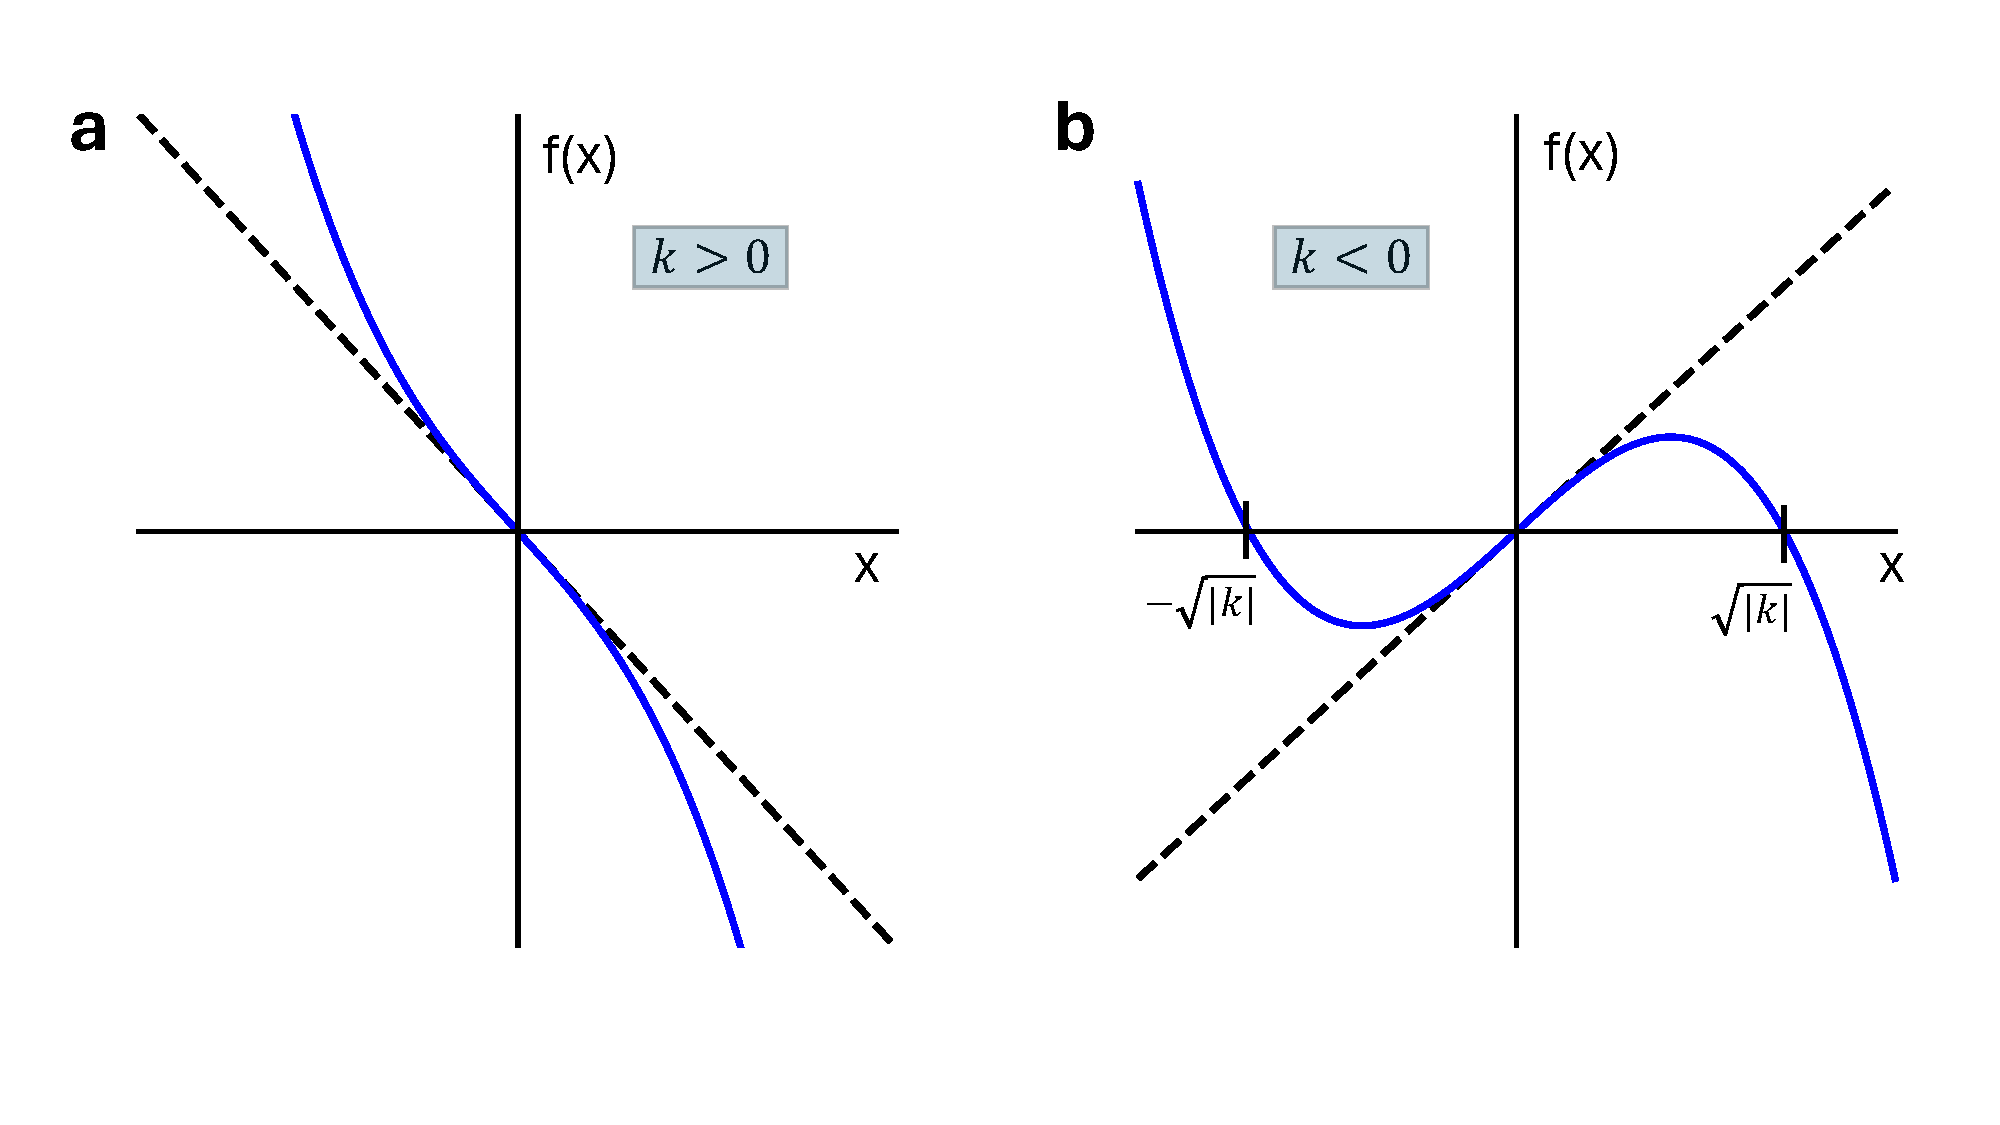
\includegraphics[width=0.8\linewidth]{bilder/kraft.pdf}
    \caption{Skizze der verwendeten Federkraft $f(x)$ in
    Abhängigkeit der Auslenkung $x$ für den Fall einer positiven
    Federkonstante $k>0$ (links) und einer negativen Federkonstante $k<0$
    (rechts). Die gestrichelte Linie zeigt einen linearen Kraftverlauf
    $f(x) = -kx$.  Im Falle einer positiven Federkonstante (links)
    entspricht dies dem Hooke'schen Gesetz und führt zu einem stabilen
    Gleichgewicht, da eine positive Auslenkung der Feder zu einer
    negativen Kraft führt und umgedreht. Im Falle einer negativen
    Federkonstante ist das Gleichgewicht $x=0$ instabil und eine leichte
    Auslenkung der Feder führt zu einer unendlich großen Auslenkung. Um
    diese Instabilität zu vermeiden, verwenden wir die Kraft $f(x) = -kx -
    x^3$ (blaue durchgezogene Linie). Im Falle von $k>0$ führt dies zu
    einem leicht nichtlinearen Kraftverlauf, aber immer noch stabilem
    Gleichgewicht (links). Für $k<0$ ist das Gleichgewicht immer noch
    instabil, aber für große Auslenkungen $|x| > \sqrt{|k|}$ wirkt die
    Kraft stabilisierend}
    \label{fig:force}
\end{figure}

\begin{figure}[h!]
    \centering
    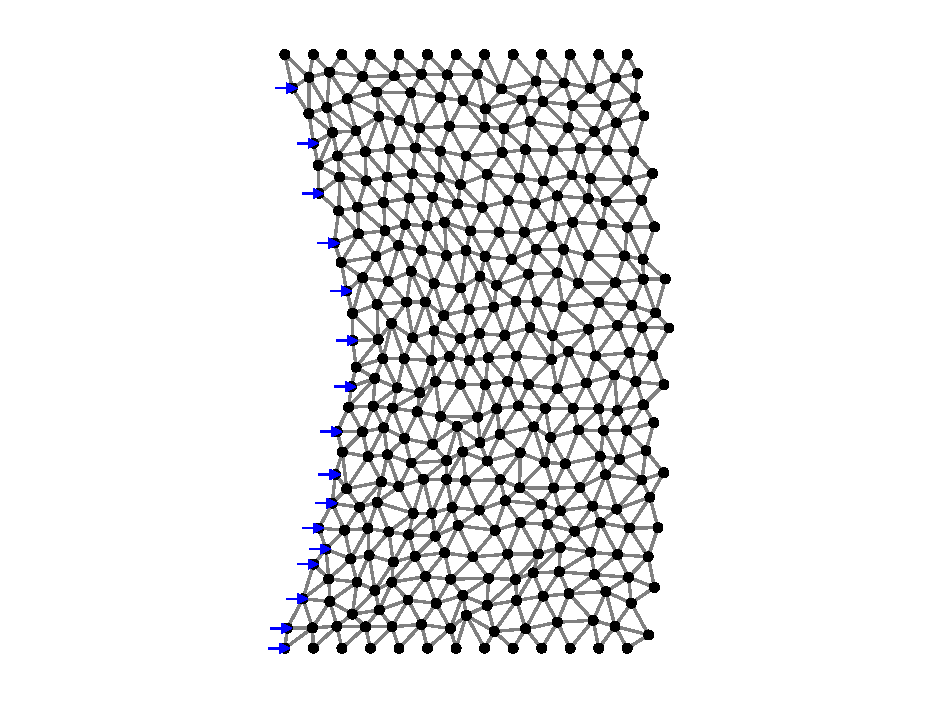
\includegraphics[trim=0cm 0.8cm 0cm 0.8cm, clip]{bilder/test4.pdf}
    \caption{Typischer Aufbau eines MMNs. Dieses besteht aus Neuronen (schwarze Kreise), die durch Federn (schwarze Linien) verbunden sind. Die Neuronen am oberen und unteren Ende sind mechanisch fixiert und können sich nicht bewegen.
    Die blauen Pfeile stellen die Krafteinwirkung auf die Neuronen dar.
    %Abbildung eines MNNs mit positiven Federkonstanten, auf das eine Kraft nach rechts ausgeübt wird.
    }
    \label{fig:positive_springs}
\end{figure}

Da wir die MNNs jedoch im 2-dimensionalen Raum simulieren wollen, müssen wir die Beschleunigung auch als 2-dimensionalen Vektor angeben, indem wir die Kraft noch mit einem normierten Richtungsvektor multiplizieren, der die Richtung der Feder und demnach auch der Kraft beschreibt. 
Weiterhin müssen alle Kräfte, die auf ein Neuron wirken, aufsummiert werden.
Die vollständige Differenzialgleichung lautet also:

{\[
    m \ddot{\vec{x}}_{i} = \sum_{j \in \textrm{NN}(i)} \left( F\left(\Delta x_{ij} - l, k_{ij}\right)
     * \frac{\vec{\Delta x_{ij}}}{ \Delta x_{ij}} \right)
     - \gamma \dot{\vec{x}}_i + \vec{F}_{\textrm{ext}, i}
\]}

Hier ist $ \vec{\Delta x}_{ij} = \vec{x}_i - \vec{x}_j$, also der Abstandsvektor zweier Neuronen,
$\Delta x_{ij}= \| \vec{\Delta x}_{ij} \|$, $l$ die Ruhelänge der Feder, 
$\vec{F}_{\textrm{ext}, i}$ die externe Kraft auf Neuron $i$ und die Summe läuft über die nächsten Nachbarn $j = \textrm{NN}(i)$ des Neurons. 

%{\[
%    \ddot x = \sum k * \Delta x * \frac{\vec{v}}{\| \vec{v} \|}
%\]}
%Die vollständige Differenzialgleichung lautet also:


%{\[
%    \ddot x_{i} = \sum_{j \in \textrm{neighbors(i)}} (-k * \Delta x -  \Delta x^3) * \frac{\vec{v_{ij}}}{\| \vec{v_{ij}} \|}
%\]}

\subsection{Optimierungsverfahren von MNNs}

Um ein MNN zu optimieren, benötigt man zuerst einmal einen Trainingsdatensatz an verschieden Verhaltensweisen, welche erlernt werden sollen. In unserem Fall besteht ein Verhalten aus den Kräften, die auf die Neuronen in der ersten Schicht wirken, und die Änderungen der Positionen der Neuronen in der letzten Schicht, die durch die gegeben Kräfte bewirkt werden sollen. Mithilfe eines Trainingsdatensatzes lässt sich nun auch bestimmen, wie gut ein Modell die Verhaltensweisen umsetzt, indem man die Entfernung jedes Neurons zu den in den Trainingsdaten gegebenen Positionen berechnet und für alle Neuronen aufsummiert. Man berechnet also die Abweichungen der Neuronen zu den Trainingsdaten. Zuletzt wird diese Abweichung noch quadriert. Diese Verfahren nennt sich \feng{mean squared error} (MSE).

\subsubsection{Genetische Algorithmen}

Genetische Algorithmen können MNNs optimieren, indem sie sich an Ideen der Evolution orientieren \cite{gentisch}. Mehrere MNNs bilden eine Population ab.
Der genetische Algorithmus beginnt damit, jedem MNN der Population einen \feng{score} zu geben, welcher beschreibt, wie gut dieses MNN die Trainingsdaten abbilden kann. Das Ziel ist es, diese Zahl zu minimieren.
Die besten MNNs werden ohne Mutation direkt an die nächste Generation übergeben.
Anschließend wird der Rest der folgenden Population durch \feng{crossover} bestimmt. Dies funktioniert, indem zwei MNNs aus der Population ausgewählt werden, wobei bessere MNNs eine höhere Wahrscheinlichkeit haben, ausgewählt zu werden.
Die Federkonstanten der beiden ausgewählten MNNs werden beim \feng{crossover} genutzt, um ein neues MNN zu erstellen, das Federkonstanten beider \enquote{Elternteile} besitzt.
Am Ende einer Iteration werden noch zufällige Mutationen vorgenommen. Die Stärke dieser Mutation nennt sich Lernrate.
Dieses Verfahren wird solange wiederholt, bis ein zufriedenstellendes MNN gefunden wurde.

\subsubsection{Partial Pattern Search}

Bei dem von \lee{} verwendeten \feng{partial pattern search} (PPS) Verfahren werden zu Beginn alle Federkonstanten auf den gleichen voreingestellten Wert gesetzt, hierfür  haben wir den von \lee{} verwendeten Wert von \num{1,15} %TODO: Einheit
übernommen.
Weiter gibt es zu Beginn eine festgesetzte Änderungsrate von 1.
Nun wird in zufälliger Reihenfolge zu jeder Federkonstante die aktuelle Änderungsrate addiert. Falls der MSE mit der veränderten Federkonstante nicht niedriger ist als vorher, wird die Änderung rückgängig gemacht.
Sollte es in einem Durchlauf aller Federkonstanten keine Verbesserung des MSE gegeben haben, wird das Vorzeichen der Änderungsrate umgekehrt und, falls diese bereits negativ war, um \SI{10}{\percent} gesenkt. Mit den genannten Werten wäre die Entwicklung der Änderungsrate also $1 \rightarrow -1 \rightarrow 0.9 \rightarrow -0.9 \rightarrow 0.81 \dots$
Dies wird für eine vorgegebene Anzahl an Wiederholungen durchgeführt, wobei eine Wiederholung nicht einen Durchlauf aller Federkonstanten, sondern die Anwendung der aktuellen Änderungsrate auf eine einzelne Federkonstante bezeichnet.

% \section{Forscherfrage}

% Ziel des Projektes ist es, ein neues Optimierungsverfahren für das Trainieren von MNNs zu entwickeln, sowie dieses mit den beiden im Artikel verwendeten Verfahren -- ein evolutionärer Algorithmus und Partial Pattern Search -- zu vergleichen.

% Ziel des Projektes ist es nicht, ein MNN selbst mechanisch umzusetzen.
% Es wird davon ausgegangen, dass 
% \begin{enumerate}
%     \item ein Vergleich der Verfahren in einer Simulation auch für das physische Trainieren der mechanischen Netzwerke aussagekräftig sein könnte und
%     \item ein \enquote{Vortrainieren} eines physischen MNN mit einer Simulation die Gesamtzeit zum Trainieren verkürzt und somit Optimierungsverfahren, auch wenn sie nur in einer Simulation verwendet werden, von Nutzen sind.
% \end{enumerate}

\newpage

\section{Vorgehensweise}

\subsection{Materialien}
\begin{itemize}
    \item Laptop (i7-11800H, 16\,GB, RTX 3060)
    \item Julia
    \begin{itemize}
        \item DifferentialEquations.jl und LinearAlgebra.jl für Autodifferenzierung der Simulation des Federsystems
        \item Graphs.jl und MetaGraphsNext.jl für Modellierung des Netzwerks als Graph
        \item Plots.jl, GLMakie.jl und Observables.jl für Visualisierung
        \item CSV.jl und Statistics.jl für Speicherung und Verarbeitung von Versuchsergebnissen
    \end{itemize}
\end{itemize}

\subsection{Methoden}

Als erstes war die Umsetzung der Simulation notwendig. Nach Herleitung der Differentialgleichung \sectionautorefname{sec:MNN-sim} haben wir diese zunächst mit dem Eulerverfahren %TODO: spezifizieren
gelöst, und konnten so zumindest visuell die Funktionsweise bestätigen. Doch das Eulerverfahren ist nicht sehr praktikabel, da man zwischen großen Zeitschritten mit kumulativen Ungenauigkeiten und kleinen Zeitschritten mit langer Laufzeit wählen muss. Deshalb haben wir danach die Julia-Bibliothek DifferentialEquations.jl verwendet, welche automatisches Lösen von Differntialgleichungen mit verschiedenen Algorithmen bietet. Wir haben die in der Dokumentation empfohlene Kombination von Tsit5 (basierend of Ch. Tsitouras' Runge-Kutta-Verfahren Verfahren aus 2011 \cite{Tsit5}) mit Rosenbrock23 verwendet, welche ähnliche Ergebnisse zu dem Euler-Verfahren mit sehr geringen Zeitschritten liefert, jedoch gleichzeitig deutlich schneller ist (ca. \SI{60}{\milli\second} vs. ca. \SI{500}{\milli\second} für 100 Sekunden simulieren). %TODO
Diese Kombination haben wir für alle Ergebnisse und Analysen verwendet und werden wir als Tsit5 abkürzen.

Um zu testen, wie gut sich ein MNN mit den verschiedenen Algorithmen optimieren lässt, wird zuerst eine Architektur für die MNNs benötigt.
In diesem Projekt wurde eine bereits vorgeschlagene Struktur verwendet \cite{Lee2022}, damit eine bessere Vergleichbarkeit zu den bereits gefundenen Ergebnissen besteht.
Dabei werden die Neuronen in gleichseitigen Dreiecken angeordnet und verbunden.
Diese Dreiecke werden in einem Gitter zusammengebracht, welches oben und unten fixiert ist.
Die auf das System einwirkenden Kräfte greifen an der linken Seite des MNNs an und die gewünschten Veränderungen finden auf der rechten Seite statt.
Diese Architektur wurde nicht dafür entwickelt, ein reales Szenario, in dem MNNs eingesetzt werden könnten, zu simulieren, sondern dient dazu verschiedene Optimierungsalgorithmen mit einer vereinfachten Problemstellung zu testen und zu verstehen, bevor man sie einsetzt.

Für eine systematische Analyse müssen zusätzlich zu der Architektur der MNNs auch die verschiedenen Verhaltensweisen festgelegt werden.
Dafür nutzen wir zufällig generierte Vektoren für die einwirkenden Kräfte (Kraftvektoren) sowie die gewünschten Positionsänderungen in der letzten Schicht (Zielvektoren).
% Jedes Neuron der letzten Schicht hat dabei ein \SI{50}{\percent} Chance, dass der Zielvektor $\begin{pmatrix} 0 \\ 0 \end{pmatrix}$ ist, es also trotz der einwirkenden Kräfte auf der Stelle bleiben \enquote{soll}.
% Bei den Kraftvektoren hat jedes Neuron der ersten Schicht eine \SI{50}{\percent} Chance, keine einwirkende Kraft zu haben, jedoch gibt es immer mindestens einen Kraftvektor.
Die Kraftvektoren werden während jedem Simulationsschritt auf die entsprechenden Neuronen angewendet, die Zielvektoren legen die Zielpositionen ausgehend von der ursprünglichen Startposition fest. %TODO: Dopplung?

Bei diesem Vorgehen sind unmögliche Kombinationen von Verhaltensweisen möglich, z.B. entgegengesetzte Positionsänderungen bei gleichen einwirkenden Kräften (s. Abb. \ref{fig:impossibletraining} (a)).
Um dies zu verhindern, überprüfen wir beim Generieren mehrerer Verhaltensweisen, dass für ein Neuron der gerade zufällig generierte Kraft- / Zielvektor mit allen anderen Vektoren für dieses Neuron mindestens einen vorgegebene Mindestwinkel bildet. 
Sollte dies nicht zutreffen, wird der Vektor neu erstellt.
Für das Generieren von Verhaltensweisen gibt es so drei Parameter:

\begin{itemize}
    \item Der Mindestwinkel zwischen Vektoren
    \item Die Skalierung der Länge der Kraftvektoren
    \item Die Skalierung der Länge der Zielvektoren
\end{itemize}

\begin{figure}[htb]
    \centering
    \scalebox{0.8}{
    \subfloat[]{
    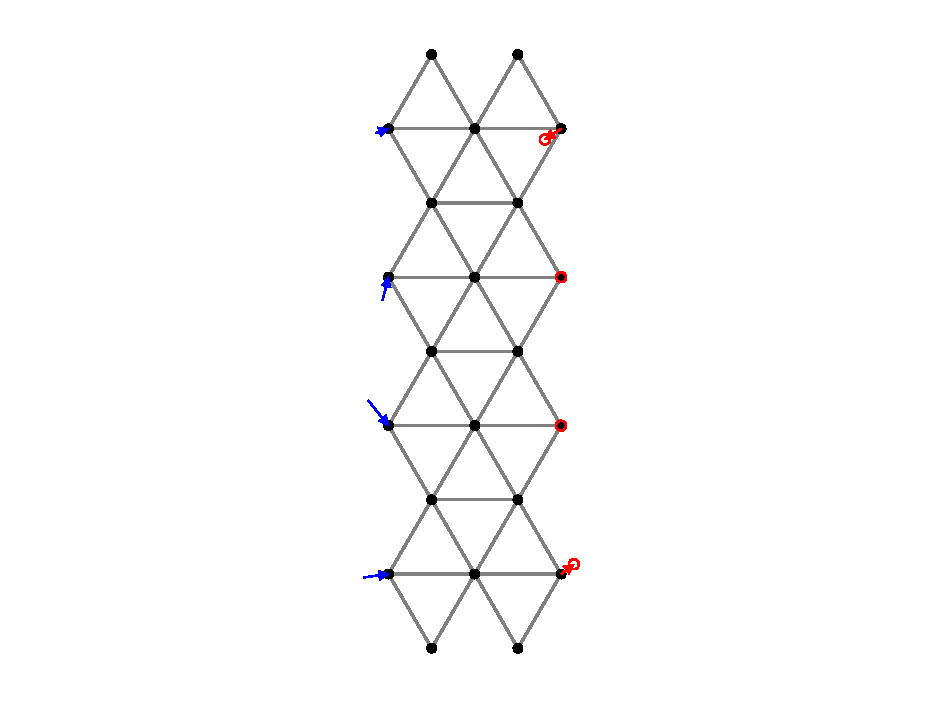
\includegraphics[trim=6cm 0.75cm 6cm 0.75cm, clip]{bilder/impossibleA.pdf}
    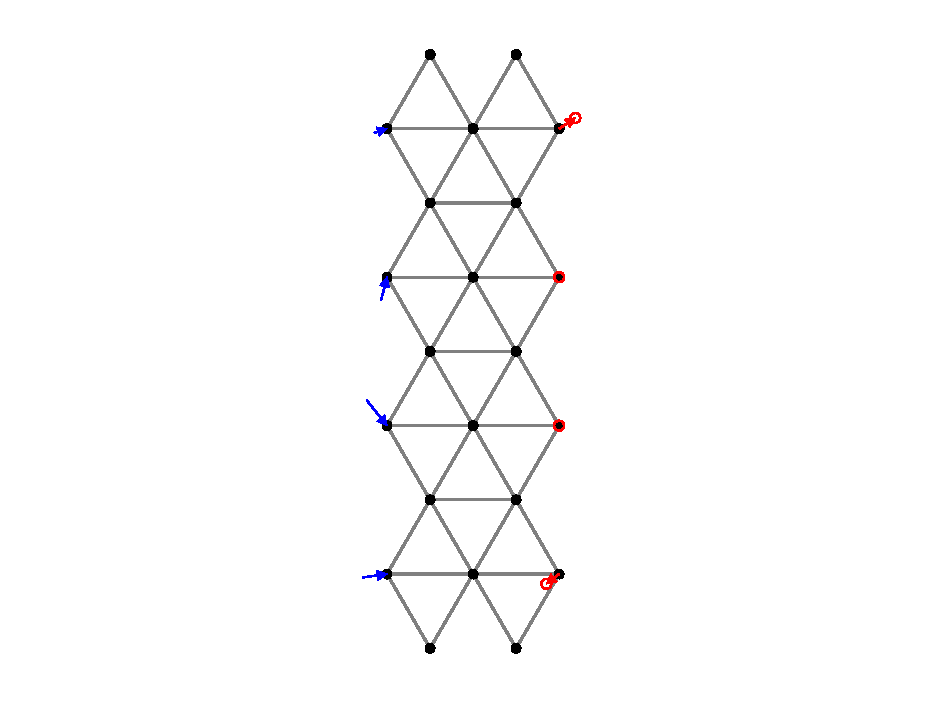
\includegraphics[trim=6cm 0.75cm 6cm 0.75cm, clip]{bilder/impossibleB.pdf}
    }
    \hspace{4em}
    \subfloat[]{
    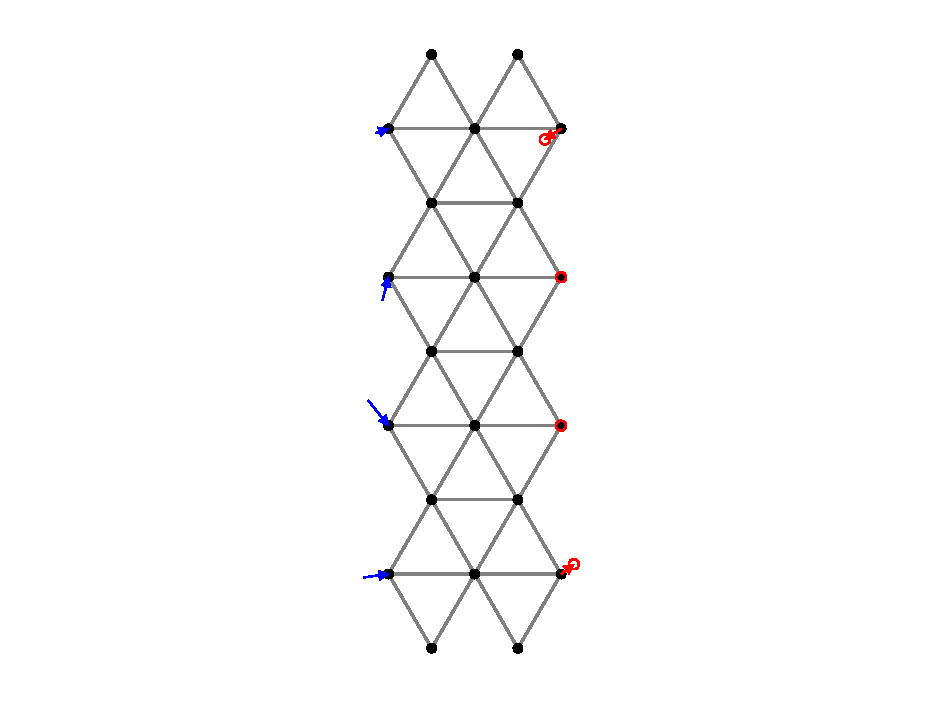
\includegraphics[trim=6cm 0.75cm 6cm 0.75cm, clip]{bilder/impossibleA.pdf}
    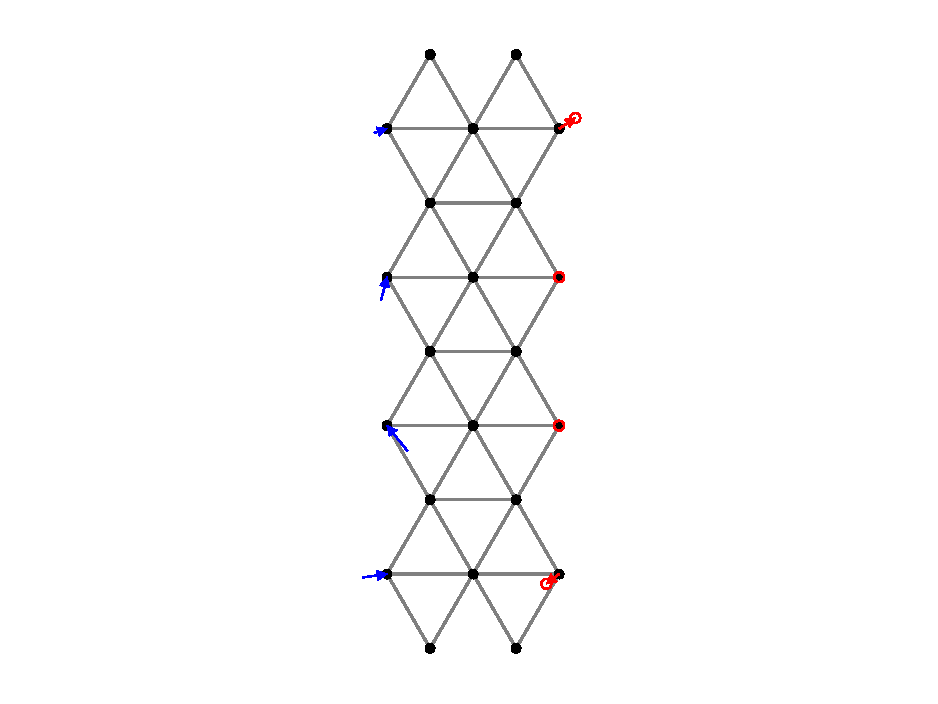
\includegraphics[trim=6cm 0.75cm 6cm 0.75cm, clip]{bilder/impossibleC.pdf}
    }
    }
    \caption{Die schwarzen Punkte sind die Neuronen, die schwarzen Verbindungslinien die Federn. Die obersten und untersten zwei Neuronen sind jeweils fixiert. Die Länge der Kraftvektoren (blau) wurde für bessere Erkennbarkeit verzehnfacht. \\
    \textbf{(a)} Zwei Verhaltensweisen, die gemeinsam unmöglich erfolgreich anzutrainieren sind. Bei beiden sind die Kraftvektoren gleich, die Zielpositionen (rote Kreise) unterscheiden sich jedoch. \\
    \textbf{(b)} Zwei Verhaltensweisen, deren gemeinsames Antrainieren möglich sein könnte, bei uns jedoch nicht vorkommen könnten, da mindestens ein Neuron der ersten Schicht (z.B. erstes von unten) in beiden Verhaltensweisen den gleichen Kraftvektor hat. Somit beträgt der Winkel zwischen diesen \ang{0} und ist entsprechend nie größer als der Mindestwinkel. Im Unterschied zu (a) wurde jedoch der Kraftvektor eines Neurons (rechtes Netzwerk, zweites von unten) verändert.}
    \label{fig:impossibletraining}
\end{figure}

Dieses Vorgehen verhindert zwar unmögliche Szenarien, schließt jedoch auch womöglich schwere, aber nicht unmögliche Kombinationen von Verhaltensweisen aus (s. Abb. \ref{fig:impossibletraining} (b)), 
%TODO: Diskussion?
zu Beginn sollte es jedoch zum Vergleichen der Optimierungsalgorithmen reichen.
% Wenn erfolgreiches Training mit den aktuellen Verhaltensweisen möglich ist, dann werden wir auch schwerer Verhaltensweisen einbringen.

% \begin{figure}
%     \centering
%     \scalebox{0.8}{
%     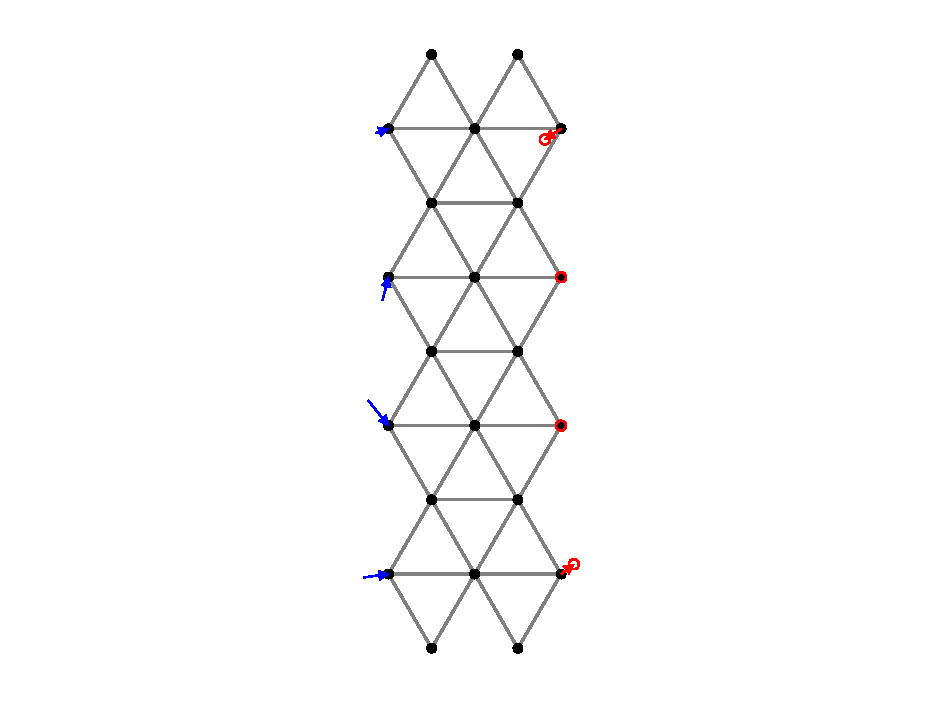
\includegraphics[trim=6cm 0.75cm 6cm 0.75cm, clip]{bilder/impossibleA.pdf}
%     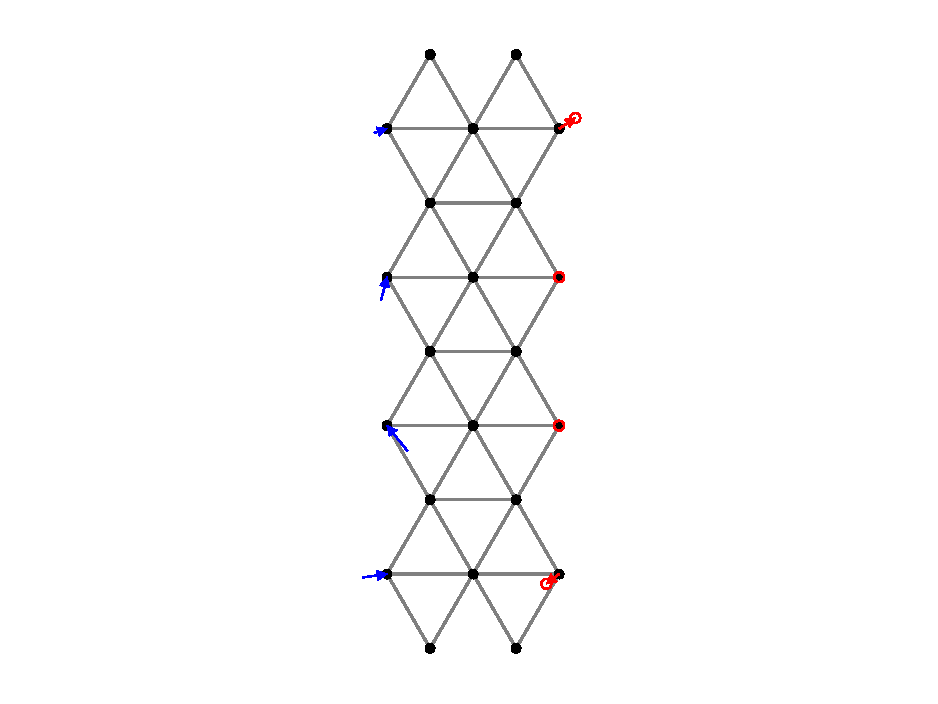
\includegraphics[trim=6cm 0.75cm 6cm 0.75cm, clip]{bilder/impossibleC.pdf}
%     }
%     \caption{Zwei Verhaltensweisen, deren gemeinsames Antrainieren möglich sein könnte, bei uns jedoch nicht vorkommen könnten, da mindestens ein Neuron der ersten Schicht (z.b. erstes von unten) in beiden Verhaltensweisen den gleichen Kraftvektor hat. Somit beträgt der Winkel zwischen diesen \ang{0} und ist entsprechend nie größer als der Mindestwinkel. Im Unterschied zu Abbildung \ref{fig:impossibletraining} wurde jedoch der Kraftvektor eines Neurons (rechtes Netzwerk, zweites von unten) verändert. Die Länge der Kraftvektoren wurde für bessere Erkennbarkeit verzehnfacht.}
%     \label{fig:notimpossibletraining}
% \end{figure}

Der von uns geschriebene Quellcode lässt sich auf höchster Ebene in zwei Teile aufteilen: Unser Paket MNN.jl mit der Implementierung des MNN und der Optimierungsverfahren sowie das Skript Compare.jl für das programmatische Testen und Vergleichen verschiedener Hyperparamerter.
Unter Hyperparameter verstehen wir einen Parameter, welcher nicht Teil des Netzwerks ist (also z.B. keine Federkonstanten), sondern die Struktur sowie das Training dieses Netzwerks beeinflusst (z.B. Optimierungsalgorithmus, Epochen, Mindestwinkel für Verhaltensweisen oder Dimensionen des Netzwerks). 

In Compare.jl verwenden wir CSV.jl zusammen mit DataFrames.jl, um verwendete Hyperparameter sowie den MSE und die Anzahl an bereits trainierten Epochen in CSV-Dateien für spätere Analyse und Vergleiche zu speichern. 
Das Speichern erfolgt dabei alle fünf Epochen.

Mithilfe von Multithreading werden außerdem mehrere Netzwerke gleichzeitig trainiert, teilweise auch mit gleichen Hyperparametern, da ein einzelner Versuch einer Hyperparameterkombination nicht sehr aussagekräftig wäre, v.a. wenn man die Verwendung von Zufallszahlen bei Erstellung von Verhaltensweisen und den Optimierungsalgorithmen bedenkt.

Da so eine Unterscheidung verschiedener Versuche auf Basis anderer Hyperparameter nicht möglich ist, wird jedem neuen Netzwerk eine UUID (\eng{universally unique identifier})
% , erstellt mit der \mintinline{julia}{uuid1()} Funktion der Random.jl-Bibliothek, 
zugeordnet und diese ebenfalls gespeichert.
Andernfalls wäre zum Beispiel das Erstellen des MSE-Verlaufs eines einzelnen Netzwerks über Epochen hinweg nicht möglich.
Diese UUID wird weiter als Startwert für den Zufallszahlengenerator gesetzt, sodass die Versuche reproduzierbar sind.

Insgesamt werden in Compare.jl zum Vergleichen für jedes Netzwerk alle fünf Epochen folgende Daten gespeichert:

\begin{itemize}
    \item aktuelle Zeit
    \item UUID
    \item Gesamtzahl an Trainingsepochen seit Erstellung
    \item Anzahl an Reihen und Spalten des Netzwerks
    \item Anzahl an Verhaltensweisen
    \item oben genannte Parameter für Erstellung der Verhaltensweisen (Mindestwinkel, Skalierungen)
    \item Art der Simulation (Eulerverfahren vs. Tsit5) %TODO: korrekt?
    \item wie viele Sekunden die Simulation jeweils maximal läuft
    \item Mutationsstärke (falls genetischer Algorithmus)
    \item MSE des Netzwerks
\end{itemize}

% \begin{figure}
%     % \centering
%     \filepath{src/}
    
%     \hspace{4em}\filepath{MNN.jl} Hauptpaket, untergeordnete Dateien werden mithilfe von \mintinline{julia}{include(path)} eingefügt 
    
    
%     \caption{Caption}
%     \label{fig:enter-label}
% \end{figure}

Bei den verschieden Testdurchläufen werden immer unterschiedliche Kombinationen von Anzahl der Reihen, Anzahl der Spalten, Anzahl der Verhaltensweisen und den unterschiedlichen Optimierungsalgorithmen festgelegt und der MSE des Netzwerks wird im Verhältnis zur Trainingszeit gespeichert. Mithilfe dieser Daten können nun statistische Analysen durchgeführt werden, um ein besseres Verständnis über die Auswirkungen dieser Eigenschaften zu erlangen.

\subsubsection{Optimierung der Ressonanzkurven}

Wenn man die bereits beschriebenen Ressonanzkurven optimieren möchte ...

\subsubsection{Backpropagation}

Backpropagation ist ein zentrales Konzept in der Funktionsweise von ANNs.
Es handelt sich dabei um einen iterativen Optimierungsalgorithmus, der verwendet wird, um die Gewichtungen der Verbindungen zwischen den Neuronen im Netzwerk anzupassen und somit die Leistung des Netzwerks zu verbessern \cite{brotcrunsher:backwardpass}. Da wir uns in unseren vergangenen Jugend forscht Projekten schon mit ANNs auseinandergesetzt haben, ist uns die Idee gekommen, diesen Algorithmus auch für MNNs umzusetzten.

Der Prozess beginnt mit der Vorwärtspropagation, bei der Eingabedaten durch das Netzwerk fließen und eine Ausgabe erzeugt wird. Der erzeugte Ausgabe-Fehler wird dann durch den Vergleich mit den gewünschten Ausgabewerten berechnet. Im nächsten Schritt wird der Fehler rückwärts durch das Netzwerk propagiert, um die Beiträge jedes Neurons zur Fehlerentstehung zu quantifizieren.
Die Gewichtungen werden entsprechend des Fehlers angepasst, um diesen zu minimieren.

Um diesen Algorithmus für MNNs zu nutzen, benötigt man zum einen eine Möglichkeit, den Fehler durch das Netzwerk zu propagieren, und zum anderen ein Verfahren, das die Federkonstanten anpasst, um den Fehler jedes einzelnen Neurons zu minimieren.
Der Fehler der Neuronen in der letzten Schicht kann einfach mit den Trainingsdaten bestimmt werden. Die Fehler in den Positionen aller anderen Neuronen sind dann der Durchschnitt der Fehler aller Neuronen, mit denen sie verbunden sind. Um herauszufinden, wie wir die Federkonstante einer Feder ändern müssen, damit die Position des Zielneurons einen kleineren Fehler bekommt, muss man erst einmal bestimmen, was der Winkel zwischen dem Fehlervektor und dem Vektor zwischen den beiden Neuronen der Federn ist. Wenn dieser zum Beispiel 90° beträgt, ist eine Änderung der Federkonstante nicht notwendig, da die Kraft den Fehler aufgrund ihrer Richtung nicht beeinflussen kann. Wenn dieser Winkel 0° beträgt, wollen wir die Federkonstante stark erhöhen, da die Kraft der Feder genau mit der Richtung des Fehlers übereinstimmt und wir das Neuron deswegen stärker entlang dieser Richtung bewegen wollen, was durch mehr Kraft erfolgt, wofür wir eine größere Federkonstante benötigen. Wenn der Winkel 180° beträgt, wollen wir die Federkonstante senken, da die Kraft genau in die falsche Richtung ausgeübt wird.

Allgemein wird die Federkonstante also um den folgenden Term erhöht:
{\[
    \frac{\vec{v_1} \cdot \vec{v_2}}{\| \vec{v_1} \| * \| \vec{v_2} \|} * \epsilon
\]}

wobei $v_1$ der Fehler eines Neurons, $v_2$ die Differenz der Positionen der beiden Neuronen einer Feder und $\epsilon$ die Lernrate ist.

Leider ist es uns nicht gelungen, ein MNN mithilfe von Backpropagation zu trainieren, da der MSE nicht signifikant gesunken ist.
Dies könnte zum einen daran liegen, dass Backpropagation voraussetzt, dass die Daten (oder Kräfte) nur in eine Richtung weitergegeben werden können, was bei MNNs nicht der Fall ist.


\newpage

\section{Ergebnisse}

Wie man in Abb. \ref{fig:ppsepochs} und Abb. \ref{fig:succes} sehen kann, kann man ein MNN mithilfe von PPS erfolgreich trainieren. Dabei fällt der MSE immer langsamer und kann nur noch durch viel Rechenzeit signifikant weiter gesenkt werden. Diese 500 Epochen, welche mit 14 verschiedenen Konstellationen von jeweils 3 verschiedenen Verhaltensweisen trainiert wurden, dauerten auf unserer Hardware ungefähr 14 Minuten. Das heißt, dass wir pro Verhaltensweise und Epoche ungefähr 0,04 Sekunden benötigen.

\begin{figure}[H]
    \centering
    \pgfplotstableread[col sep=comma]{bilder/PPSEpochs.csv}\Data
    \begin{tikzpicture}
        \begin{axis}[%xtick=data, 
        yticklabel style={
            /pgf/number format/precision=2,
            /pgf/number format/fixed,
        },
        xlabel={Epochen},
        ylabel={MSE},
        width=0.9\textwidth,
        height=6cm,
        xmin=5,
        xmax=505,
        title={MSE-Verlauf von PPS}
        ]
        \addplot [only marks]
            plot [mark size=1pt]
            table [x=epochs, y=loss_mean] {\Data};
        \end{axis}
    \end{tikzpicture}
    \caption{Die Punkte stellen den Mittelwert des MSE von 14 Netzwerken (alle verschiedene UUID) nach einer bestimmten Epochenzahl dar. Das Netzwerk wurde mit PPS trainiert und zur Simulation wurde das numerische Lösen genutzt, alle Hyperparameter sind identisch. Originaldaten sind im Repository \cite{RepoMNN} in der Datei \filepath{src/data/PPSNumBehaviours\_2024-01-14T13:56:06.441.csv} zu finden. Der Mittelwert des MSE vor dem Training (0 Epochen) ist $\approx \num{0.968}$ und wurde für bessere y-Achsenskalierung entfernt.}
    \label{fig:ppsepochs}
\end{figure}

Das Training mit dem genetischen Algorithmus ist im Gegensatz zu PPS nicht erfolgreich gewesen.
Nach 200 Epochen lag der minimale MSE bei ungefähr \num{0.55} (s. Abb. \ref{fig:evolutionepochs}).
Dort befand er sich jedoch auch schon nach 80 Epochen, der MSE des Netzwerk befindet sich also in einem lokalem Minimum.
Mit der aktuellen hohen Lernrate von \num{0.05} werden keine feineren Anpassungen an den Federkonstanten mehr vorgenommen und ein signifikant niedriger MSE kann nicht erreicht werden.
Würde jedoch eine kleinere Lernrate gewählt werden, würden es sehr lange dauern, bis überhaupt erst dieser MSE von \num{0.55} erreicht wird.

\begin{figure}[H]
    \centering
    \pgfplotstableread[col sep=comma]{bilder/EvolutionEpochs.csv}\Data
    \begin{tikzpicture}
        \begin{axis}[%xtick=data, 
        yticklabel style={
            /pgf/number format/precision=2,
            /pgf/number format/fixed,
        },
        xlabel={Epochen},
        ylabel={MSE},
        width=0.9\textwidth,
        height=6cm,
        xmin=5,
        xmax=205,
        title={MSE-Verlauf des genetischen Algorithmus}
        ]
        \addplot [only marks]
            plot [mark size=1pt]
            table [x=epochs, y=loss_mean] {\Data};
        \end{axis}
    \end{tikzpicture}
    \caption{Die Punkte stellen den Mittelwert des MSE von 10 Netzwerken (alle verschiedene UUID) nach einer bestimmten Epochenzahl dar. Das Netzwerk wurde mit dem evolutionären Algorithmus trainiert und zur Simulation wurde das numerische Lösen genutzt, die restlichen Hyperparameter aller Netzwerke sind identisch zu den für Abb. \ref{fig:ppsepochs} verwendeten. 
    Originaldaten sind in der Datei \filepath{src/data/EvolutionEpochs\_2024-01-14T20:57:11.627.csv} zu finden. Der Mittelwert des MSE vor dem Training (0 Epochen) ist $\approx \num{0.968}$ und wurde für bessere y-Achsenskalierung entfernt.}
    \label{fig:evolutionepochs}
\end{figure}

Insgesamt lässt sich also sagen, dass in unserer Implementation PPS deutlich besser abschneidet als der evolutionäre Algorithmus, sowohl was Laufzeit als auch bisher erreichbare MSEs angeht.

Der einzige Vergleich von genetischer Optimierung und PPS, den wir finden konnten, war von \lee{}, deren Ergebnisse sich von unseren unterscheiden: Sie konnten mit dem genetischen Algorithmus einen deutlich niedrigeren MSE erreichen als mit PPS. Jedoch haben sie ersteren für mehr als 100 Stunden trainiert, und den zweiten weniger als drei Stunden \cite[Abb. 4]{Lee2022}; wie bei uns auch braucht der genetische Algorithmus deutlich länger, um die gleiche Leistung wie PPS zu erreichen.

Die Laufzeit scheint in der Tat bei PPS besser zu sein. Für eine Aussage über den niedrigsten erreichbaren MSE müssten jedoch das Problem des lokalen Minimums für den genetischen Algorithmus gelöst und beide sehr lange laufen gelassen werden. 

\begin{figure}[H]
  \centering
  \subfloat[Ein MNN, welches aus 5 Spalten und 3 Reihen besteht.]{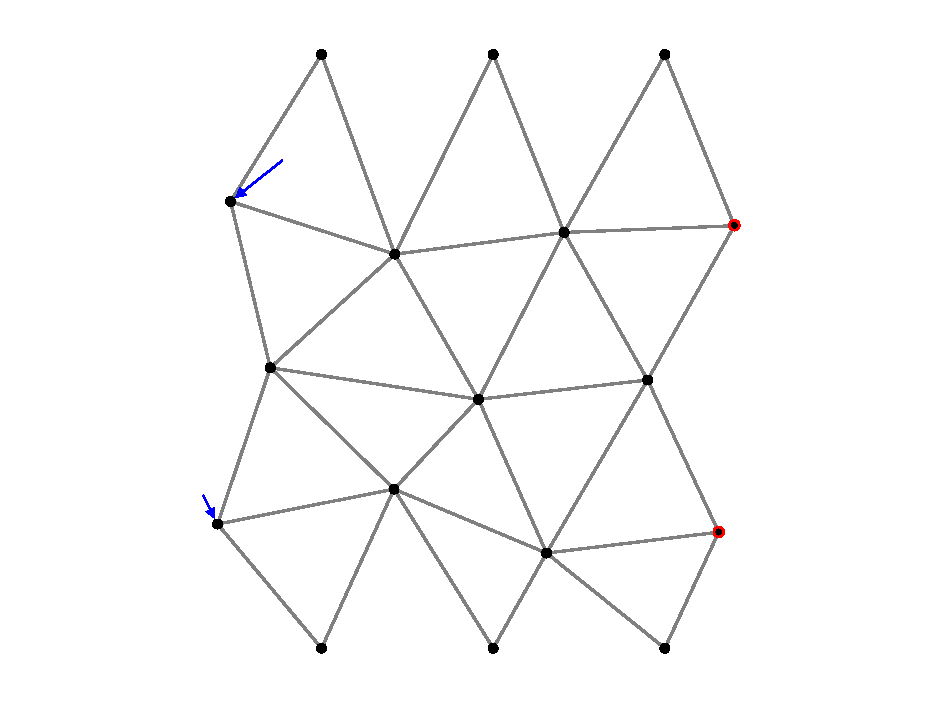
\includegraphics[width=0.35\textwidth]{bilder/test.pdf}\label{fig:f1}}
  \hfill
  \subfloat[Ein MNN, welches aus 15 Spalten und 9 Reihen besteht.]{\scalebox{0.8}{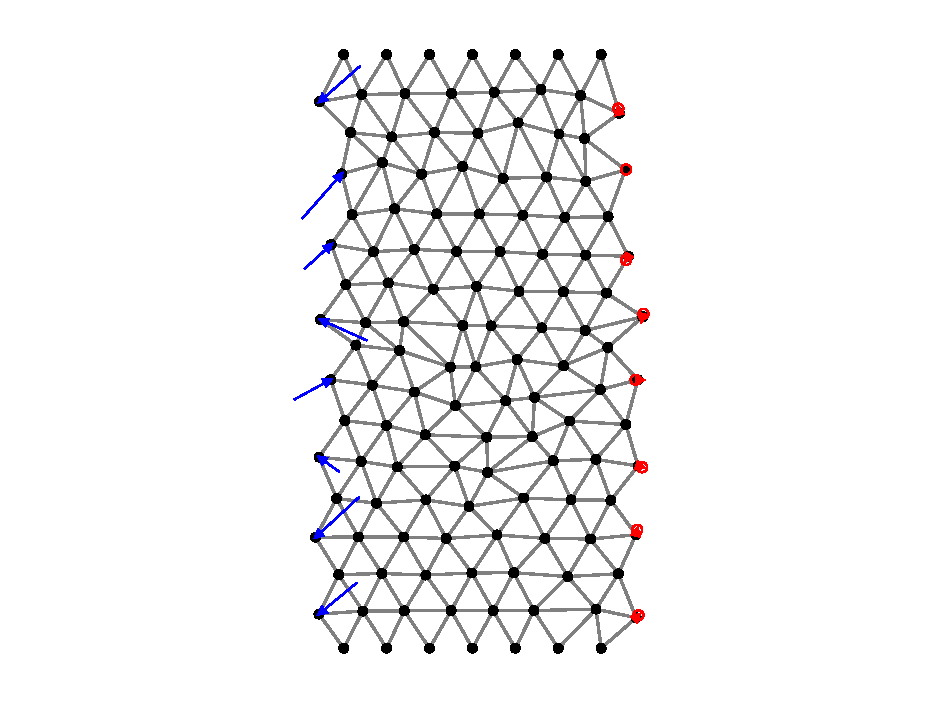
\includegraphics[width=0.65\textwidth]{bilder/test2.pdf}\label{fig:f2}}}
  \caption{Die beiden MNNs wurden jeweils mit einer Verhaltensweise mit PPS trainiert. Die Kraftpfeile sind blau eingezeichnet und die roten Kreise geben an, wo sich die Ausgabeneuronen befinden sollen. Man erkennt, dass die Netzwerke erfolgreich trainiert wurden, das sich die Neuronen in den roten Kreisen befinden.}
  \label{fig:succes}
\end{figure}


\begin{figure}[H]
    \centering
    \pgfplotstableread[col sep=comma]{bilder/PPSNumBehavioursErrorBar.csv}\Data
    \begin{tikzpicture}
        \begin{axis}[xtick=data, error bars/y dir=both, error bars/y explicit, 
        yticklabel style={
            /pgf/number format/precision=2,
            /pgf/number format/fixed,
        },
        xlabel={Anzahl an Verhaltensweisen},
        ylabel={MSE},
        title={MSE von PPS, abhängig von Anzahl an Verhaltensweisen}
        ]
            \addplot [only marks]
                plot [mark size=1pt]
                table [x=behaviours, y=loss_median, y error =var] {\Data};
        \end{axis}
    \end{tikzpicture}
    \caption{Die Punkte stellen den Median des MSE von je 30-34 verschiedenen Durchläufen und die Fehlerbalken die Standardabweichung vom Median dar. Das Netzwerk wurde 100 Epochen mit PPS trainiert und zur Simulation wurde das numerische Lösen genutzt, alle Hyperparameter außer Anzahl der Verhaltensweise sind identisch. Originaldaten sind im Repository \cite{RepoMNN} im Ordner \filepath{src/data/}: \filepath{PPSNumBehaviours\_2024-01-14T15:16:06.598.csv}, \filepath{PPSNumBehaviours\_2024-01-14T15:08:40.927.csv} und \filepath{PPSNumBehaviours\_2024-01-14T13:56:06.441.csv}}
    \label{fig:numbehaviours}
\end{figure}

\begin{figure}[H]
    \centering
    \pgfplotstableread[col sep=comma]{bilder/EvolutionNumBehavioursMedian.csv}\Data
    \begin{tikzpicture}
        \begin{axis}[xtick=data, error bars/y dir=both, error bars/y explicit, 
        yticklabel style={
            /pgf/number format/precision=2,
            /pgf/number format/fixed,
        }, xlabel={Anzahl an Verhaltensweisen}, ylabel={MSE},
        title={MSE des genetischen Algorithmus, abhängig von Anzahl an Verhaltensweisen}
        ]
            \addplot [only marks]
                plot [mark size=1pt]
                table [x=behaviours, y=loss_median, y error=var] {\Data};
        \end{axis}
    \end{tikzpicture}
    \caption{Die Punkte stellen den Median des MSE von je 15 verschiedenen Durchläufen und die Fehlerbalken die Standardabweichung vom Median dar. Das Netzwerk wurde 100 Epochen mit dem genetischen Algorithmus trainiert, die anderen Hyperparameter sind identisch zu Abb. \ref{fig:numbehaviours}. Originaldaten sind unter \filepath{src/data/EvolutionNumBehaviours\_2024-01-15T16:03:55.251.csv} zu finden.}
    \label{fig:numbehavioursevolution}
\end{figure}


\lee{} analysierten in ihrer Simulation unter anderem den Zusammenhang von MSE und Anzahl an Verhaltensweisen.
Es ist bei ihren Ergebnissen zu erkennen, dass der MSE tendenziell stark steigt, je mehr Verhaltensweisen gleichzeitig trainiert werden \cite[Abb. 5A u. 5C]{Lee2022}.
Wir konnten dieses Verhalten sowohl bei PPS als auch der evol. Opt. bestätigen (s. Abb. \ref{fig:numbehaviours} und \ref{fig:numbehavioursevolution})
% : bei PPS Bei fünf statt einer Verhaltensweise ist der MSE im Median ca. doppelt so hoch.
% Dies lässt sich durch die Erhöhung  

Weiter konnten wir den aus \cite[Abb. 5B]{Lee2022} ersichtlichen Zusammenhang bestätigen, zumindest beim Training mit PPS:
Je mehr Reihen das Netzwerk hat, desto höher der MSE, und je mehr Spalten das Netzwerk hat, desto niedriger der MSE (vgl. Abb. \ref{fig:ppsrowscols}).
Sowohl eine erhöhte Anzahl an Reihen als auch an Spalten erhöht die Menge an Federn und somit die notwendigen Schritte zur erfolgreichen Optimierung. Jedoch senkt eine höhere Anzahl an Spalten den MSE vermutlich dadurch, dass sie entlang der Kraftrichtung von links nach rechts liegen und so auch mehr Möglichkeiten zur Veränderung und Optimierung dieser bieten, während Reihen senkrecht zu dieser Richtung sind und ihre Anzahl zusätzlich proportional zur Anzahl an Kraftvektoren und Zielpositionen ist.

\begin{figure}[H]
    \centering
    \pgfplotstableread[col sep=comma]{bilder/PPSNumRowsColsMean.csv}\Data
    \begin{tikzpicture}
        \begin{axis}[
            view/h = 135,
            xlabel={Anzahl Reihen},
            x dir=reverse,
            zlabel={MSE},
            ylabel={Anzahl Spalten},
            title={MSE von PPS abhängig von Anzahl an Spalten und Reihen},
            ]
            \addplot3 [
            surf, shader=interp, mesh/cols=6,
            % mesh/ordering=y varies,
            ] table [x=rows, y=columns, z=loss_mean] {\Data};
        \end{axis}
    \end{tikzpicture}
    \caption{MSE in Abhängigkeit der Anzahl an Spalten und Reihen eines Netzwerks (niedrige MSE-Werte sind blau, hohe rot). Als Optimierungsalgorithmus wurde PPS verwendet. Pro Kombination gab es nur ein Netzwerk. Datei: \filepath{src/data/PPSNumRowsColumns\_2024-01-06T13:23:22.688.csv}}
    \label{fig:ppsrowscols}
\end{figure}

Unsere Annahme aus der Einleitung, dass wir auch durch unsere Simulation relevant Ergebnisse erzeugen können, scheint sich also zu bestätigen.
Denn wir kommen zu ähnlichen Schlüssen wie \lee{}, die ihren Simulationsalgorithmus und -ergebnisse anhand eines physischen Aufbaus bestätigen konnten.


% Eine andere Erkenntnis, welche wir durch unsere Analyse gewinnen konnten, ist das Verhältnis von dem MSE und der Anzahl der Trainingsdaten. Es lässt sich nämlich erkennen, dass es deutlich schwerer ist mehrere verschiedene Verhaltensweisen gleichzeitig zu trainieren, was in \ref{fig:numbehaviours} sehr deutlich erkennbar ist. Wenn wir mit nur 5 verschiedenen Verhaltensweisen trainieren, ist der MSE nach gleicher Anzahl von Epochen bereits ungefähr doppelt so groß, wie bei einer Verhaltensweise. Dies lässt sich durch die größere Komplexität erklären, welche durch jede neue Verhaltensweise hinzugefügt wird.


\subsection{Framework}

Die von uns geschriebene Bibliothek \cite{RepoMNN} soll nicht nur von uns leicht bedient und erweitert werden, sondern auch von anderen.
Hierzu fehlen zwar noch Dokumentation und Anleitungen, doch der Programmcode ist durch die Aufteilung der einzelnen Aufgabenbereiche und Aspekte der Bibliothek auf verschiedene Verbünde / Strukturen (s. Abb. \ref{fig:uml}) bereits entsprechend gestaltet (s. Prog. (Programmausschnitt) \ref{code:verwendung}).
Denn diese bieten gemeinsam mit den Möglichkeiten der Programmiersprache Julia, z.B.
%Julias Möglichkeiten 
der Funktionsüberladung die Option, einfach eigene Aspekte hinzuzufügen, ohne den Rest selbst schreiben zu müssen (s. Prog. \ref{code:anpassung}).

\begin{code}[1]{Beispielprogramm, welches MNN.jl verwendet}{code:verwendung}
using MNN
net = Network(5,4) # erstelle Netzwerk mit 5 Spalten und 4 Reihen

t1 = Trainer(net, PPS(), Diff(100)) # Training mit PPS und num. Simu. (100s Dauer)
t2 = Trainer(net, Evolution(), Diff(100)) # evol. Verfahren statt PPS
t3 = Trainer(net, Evolution(), Euler(100)) # Euler-Simulation statt numerisch

train!(net, 100, t1) # Training mit t1 für 100 Epochen
reset!(net) # Positionen der Neuronen zurücksetzen
# Netz + Verhaltensweise anzeigen; wird während Sim. autom. aktualisiert
vis = Visualizer(net, behaviour=t1.behaviours[1])
# 100s mit 1. Verhaltensweise simulieren
simulate!(net, Diff(100), t1.behaviours[1], vis = vis)
\end{code}

\begin{code}[1]{Verwendung von MNN.jl mit einer eigenen Simulation.
Diese kann ohne Veränderung des Quellcodes des Pakets hinzugefügt und nahtlos mit dem Rest des Pakets verwendet werden, indem der eigene Verbund als Untertyp von MNN.Simulation deklariert und die Funktion MNN.simulate! mit dem eignen Verbund überladen wird. 
Man muss also nicht noch Training, Visualisierung, MSE-Berechnung, Verhaltensweisenerstellung etc. selbst schreiben. Für das Hinzufügen eigener Trainingsverfahren und Visualisierungen wäre das Vorgehen ähnlich.
}{code:anpassung}
using MNN
mutable struct MySim <: MNN.Simulation
    modifier::Function
    # ...
end
# eigener Konstruktor; "modifier" wird später autom. von MNN.jl überschrieben
MySim(...) = MySim((net, acc) -> nothing), ...)

function MNN.simulate!(
    network::Network, sim::MySim; vis::Union{Visualizer,Nothing}=nothing
)
    # sim.modifier(net, acc), um Beschl.-vektor "acc" entspr. Kraftvektor anzupassen
    # MNN.update_positions!(vis, network), um Visualisierung zu aktualisieren
    # ...
end
# nutze MNN.jl wie üblich (s. vorheriger Programmausschnitt)
# ...
t = Trainer(net, PPS(), MySim(...))
# ...
simulate!(net, MySim(...), t1.behaviours[1], vis = vis)
# ...
\end{code}


\begin{figure}[H]
    \centering
    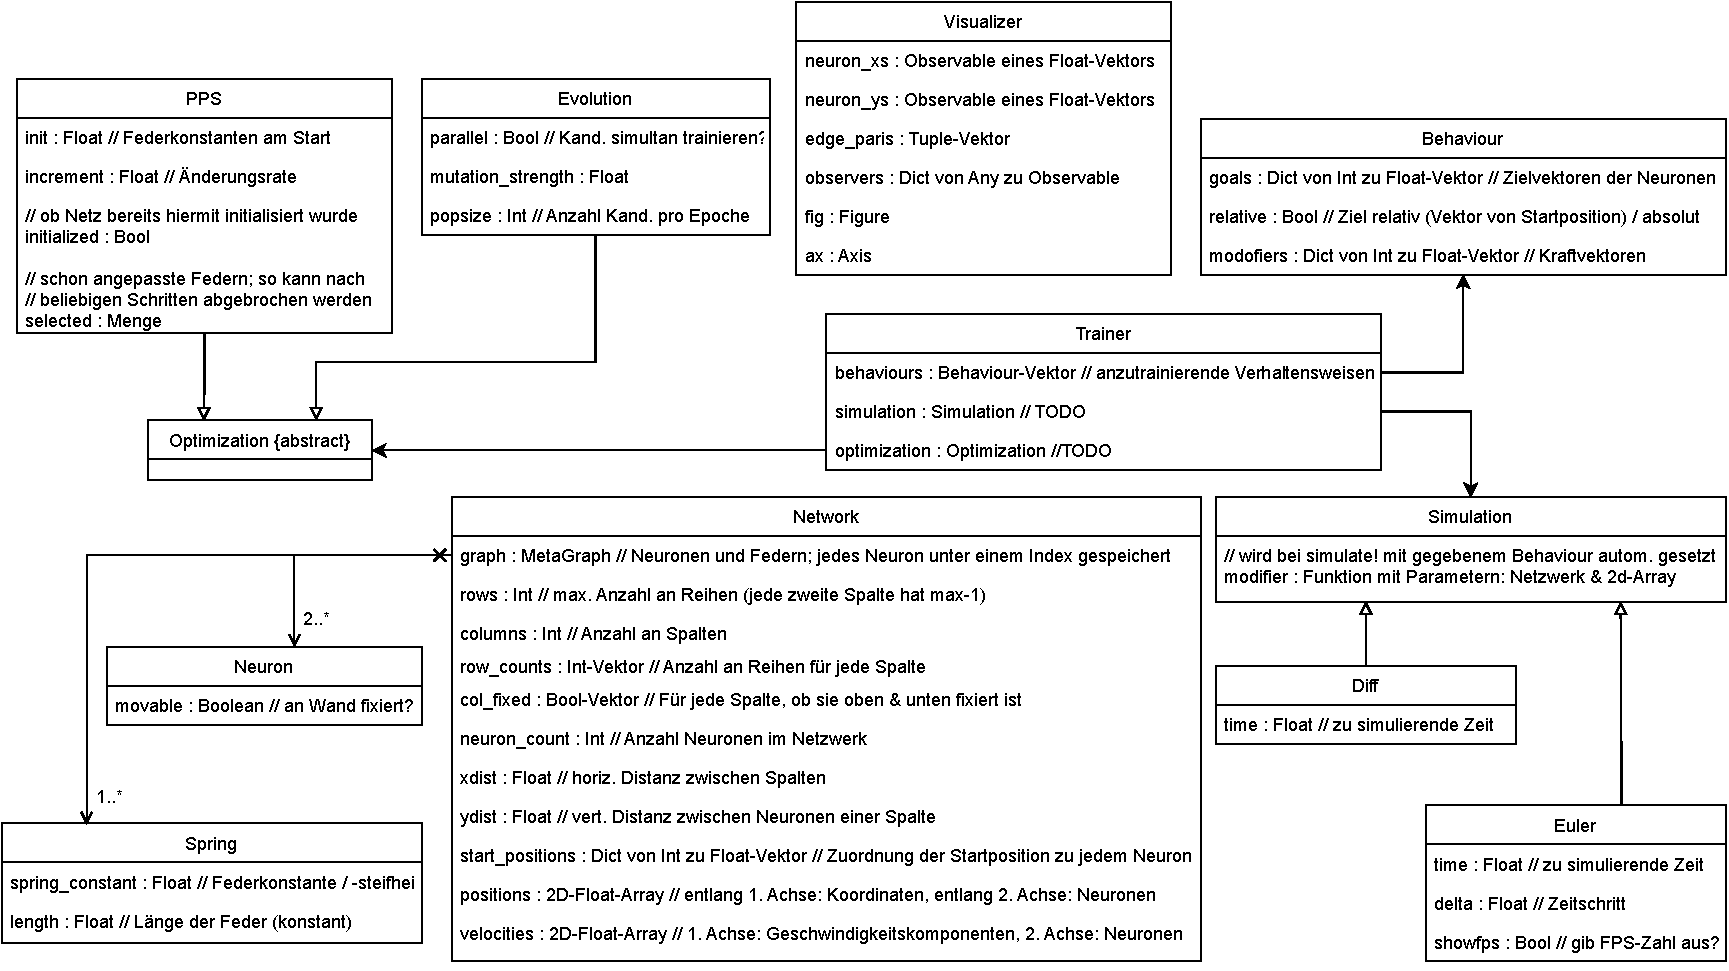
\includegraphics[width=0.9\textwidth]{bilder/UML.pdf}
    \caption{UML-Diagramm des Programm-Aufbaus. Da es sich hier um Verbünde und nicht Klassen handelt, sind die Methoden nicht mit aufgelistet.}
    \label{fig:uml}
\end{figure}

Zudem ist die von uns entwickelte Bibliothek die erste Open Source-Implementation von MNNs und wir stellen auch die ersten öffentlichen Daten von den Trainingsverläufen für weitere Analysen zur Verfügung \cite{RepoMNN}.

\section{Diskussion}

Unser neuer Optimierungsansatz, Backpropagation, war zwar nicht erfolgreich, jedoch konnten wir erfolgreich die Leistung der zwei tatsächlich verwendeten Optimierungsalgorithmen beurteilen, auch in Abhängigkeit einiger Parameter -- sie stimmen mit dem aktuellen Forschungsstand überein.

Vor allem unsere Analyse der Abhängigkeit von Spaltenanzahl, Reihenanzahl und Anzahl an Verhaltensweisen ist interessant, da diese für MNNs bisher nur in Simulationen getestet wurden.
Jedoch wurde dafür z.B. bei \lee{} immer Gradient Descent verwendet \cite[6]{Lee2022Sup}, da dies schneller ist.
Wir haben diese Tests nun direkt mit den zu untersuchenden Verfahren durchgeführt, und konnten so verfahrensbedingte Unterschiede ausschließen.
Ausnahme bildet die Analyse der Auswirkungen der Spalten- und Reihenzahl, welche aufgrund der hohen Rechenzeit bisher nur für PPS durchgeführt wurde.
Den Test mit genetischer Optimierung wollen wir als nächstes durchführen, denn er könnte weniger unter einer erhöhten Reihenanzahl leiden, da anders als bei PPS \enquote{irrelevante} Federn die Trainingszeit vermutlich nicht erhöhen würden.

Weiter wollen wir das Problem des lokalen Minimums des genetischen Algorithmus lösen, um neben der Laufzeit nun auch bestimmen zu können, welche den niedrigsten MSE erreichen kann, unabhängig von Laufzeit.
Dies wäre vor allem interessant, da \lee{} durch die stark unterschiedliche Trainingszeiten der beiden Algorithmen (über 100 Stunden vs. unter 3 Stunden) noch keine ausreichenden Daten für diesen Vergleich liefern. Zum Lösen des Problems wollen wir die Lernrate des genetischen Algorithmus adaptiv machen, sodass sie zu Beginn des Training hoch ist, um den MSE schnell zu senken, und dann immer weiter sinkt, um lokalen Minima zu entkommen.

Da wir uns momentan auf den stabilen Endzustand der MNNs beschränken, könnte man die Differenzialgleichungen stark vereinfachen, indem man nicht die Beschleunigungen, sondern die Geschwindigkeiten der Neuronen mit den auf sie einwirkenden Kräften gleichsetzt.
Dadurch würde man Schwingungen in dem Netzwerk verhindern, da sich die Neuronen einfach direkt dem Ruhezustand annähern würden, wodurch die Lösung deutlich einfacher zu beschreiben ist und höchstwahrscheinlich auch schneller berechnet werden kann. 
Wenn man bedenkt, dass wir beim Trainieren der Netzwerke fast die ganze Zeit mit der Simulation der MNNs verbringen, könnte diese Veränderung eine große Verbesserung der Performance ausmachen und so mehr Vergleiche ermöglichen, vor allem rechenzeitintensive wie der im vorletzten Absatz erwähnte.

% Das Wählen der Hyperparameter ist eine zentrale Aufgabe bei der Optimierung von MNNs und kann höchstwahrscheinlich am besten durch eine adaptive Anpassung der Parameter während des Lernprozesses gelöst werden. 
% So kann bei einem großem MSE eine höhere Lernrate für größere Veränderungen der Federkonstanten und bei einem niedrigem MSE eine relativ niedrige Lernrate für feinere und genauere Anpassungen sorgen. Eine derartige adaptive Hyperparameteranspassung haben wir jedoch noch nicht entwickelt.

Es gibt es noch weitere Hyperparameter, die wir testen möchten sowie teilweise noch den CSV-Dateien als Spalten hinzufügen müssen, wie z.B. die Trainingsparameter für die Optimierungsverfahren (Startwert und Änderungsrate für PPS, \eng{population size} und Lernrate für genetische Optimierung).

Weiter wollen wir in der Zukunft Kombinationen an Optimierungsverfahren analysieren, vor allem die Anwendung von erst PPS und dann genetischen Algorithmen.
Denn so könnte man die Geschwindigkeit von PPS nutzen, um den MSE schnell zu senken, und nach Erreichen eines lokalen Minimums einen genetische Algorithmus, um einen niedrigeren MSE erreichen zu können -- vorausgesetzt, wir können bestätigen, dass letztere niedrigere MSEs als PPS erreichen können. 

Zusätzlich zu der bereits getesteten Architektur gibt es noch viele andere interessante Möglichkeiten, ein MNN aufzubauen.
Wenn man zum Beispiel versucht, erdbebensichere Häuser und einsturzsichere Brücken durch MNNs umzusetzen, müsste man das Resonanzverhalten analysieren und untersuchen, inwiefern ein MNN auf Schwingungen reagiert.
Vielleicht ist es sogar möglich, dem System eine genaue Resonanzkurve, die erlernt werden soll, als Trainingsdaten zu geben.
Dies könnte man umsetzen, indem man den Betrag der auf das MNN einwirkenden Kraft nicht konstant gleich lässt, sondern als Sinusfunktion der Zeit angibt.
Dadurch könnte man schwingende Kräfte simulieren, welche auch Schwingungen im Netzwerk auslösen würden.
Zudem müsste man auch die Verhaltensweisen ändern, da sie zusätzlich zu der Richtung der einwirkenden Kräfte auch noch die Frequenz der Schwingung einbeziehen müssten und zudem nicht die Positionen der Neuronen als zu lernendes Kriterium für die Verlustfunktion nutzen könnten.
Vielmehr müsste sich der Verlust darauf beziehen, wie stark das System, je nach Frequenz der Schwingungen der Kraft, selber anfängt zu schwingen.
Zum Beispiel wäre es vorstellbar, so einen Resonanzverstärker für Musikinstrumente zu bauen, welcher nur auf die Frequenzen reagiert, die zu den Tönen der Tonleiter gehören.
Aber auch Flugzeugflügel könnten als MNN gebaut werden, um auf die Turbulenzen der sie umströmenden Luft passsend zu reagieren.

Weiter sollten unsere Programme ebenso mit einem dreidimensionalen MNN funktionieren.
Die Implementation wäre nicht sehr aufwändig, da keine Änderung der Formeln und nur leichte Programmänderungen notwendig wären.
Durch die höhere Komplexität könnten mehr und komplexere Verhaltensweisen gleichzeitig erlernt werden, es würde aber der Trainingsaufwand voraussichtlich sehr stark steigen.
Bisher wurden dreidimensionale MNNs trotz der Vorteile (neue Anwendungszwecke, komplexere Verhaltensweisen) weder gebaut noch simuliert.
Wir planen, es zu probieren, sobald wir mit allen Optimierungsverfahren erfolgreich zweidimensionale Netzwerke trainieren können und ihre relevanten Hyperparameter analysiert haben.

Zusammenfassend stellen MNNs eine faszinierende Möglichkeit dar, Erkenntnisse der modernen KI mit Materialforschung zu verbinden. Dieses Forschungsfeld ist gerade erst im Entstehungsprozess. Wir sehen hier eine großes Zukunftspotenzial und wollen mit unserem Projekt einen Beitrag dazu leisten.

\newpage

\section{Quellen}

\printbibliography[heading=none]

\end{document}